\documentclass[10pt]{report}

\usepackage[utf8]{inputenc}

\usepackage{makeidx}
\usepackage{mathtools}
\usepackage{amsmath}
\usepackage{amsfonts}
\usepackage{graphicx}
\usepackage{float}
\usepackage{url}

%\usepackage{biblatex}
\title{Tilted Beta Extremal Mixtures}
\author{Samuel Sekarski}
\date{June 2020}
%\makeindex
%\addbibresource{bib.bib}

\newtheorem{theorem}{Theorem}


\begin{document}
\maketitle


%\chapter*{Acknowledgements}

\tableofcontents
\listoffigures

\chapter{Introduction}
\label{sec:intro}
%Motivation, based on chapter 8 (mostly sections 8.1 and 8.2) of Coles (2001) and Boldi and Davison (2007)
%layout of project

Modelling extreme events is becoming more and more important, mostly in order to assess risks (financial, ecological, structural, $\ldots$). Modelling of univariate extremes is well documented and explored, using techniques such as block maxima, threshold exceedances and point processes.
However, things become, as usual, more complicated in higher dimensions. Multivariate extremes suffer from problems that affect univariate extremes less, such as the curse of dimensionality and sparsity.

The most primitive way to deal with multivariate extremes is to study each component as a univariate process. However, this is limiting, as we could easily imaging that there is interdependence of the components, which we lose by considering the components independently. Another reason, as is stated in \cite{Coles}, is that the combination of the individual processes might be of more interest than each process individually.

Methods analogous to block maxima and threshold analysis exist for multivariate cases and we can find models for extreme multivariate events, but we do not have a characterization for the class of all the models. Theorem 8.1 from \cite{Coles} defines a family of bivariate extreme value distributions (and can be generalized to general multivariate case) that arise as the limiting distribution for componentwise block maxima. 

Here is Theorem 8.1 restated (for a bivariate process) for completeness:

\begin{theorem}

Let $M^*_n = (\max_{i=1,...,n} \{X_i\}/n, \max_{i=1,...,n} \{Y_i\}/n)$ be the vector of rescaled componentwise maxima, where $(X_i,Y_i)$ are independent vectors with standard Fréchet marginal distributions. Then if
$$
\mathbb{P}\{M^*_n \leq (x,y) \} \xrightarrow[]{d} G(x,y),
$$
where $G$ is a non-degenerate distribution function, then $G$ has the form
$$
G(x,y) = \exp\{-V(x,y)\}, \quad x>0, y>0
$$
where
$$
V(x,y) = 2 \int^1_0 \max \left(\frac{w}{x},\frac{1-w}{y}\right)d\nu(w)
$$
and $\nu$ is a distribution on $[0,1]$ satisfying the mean constraint
$$
\int_0^1 wd\nu(w) = 1/2.
$$


\end{theorem}


The problem is that we don't know how to characterize $\nu$. An approach is to try and approximate the class arbitrarily well, using parametric subfamilies or nonparametric methods and another way is to use nonparametric methods.

Boldi and Davison \cite{BoldiDavison} approached the problem by using a semi-parametric model based on mixtures of Dirichlet distributions that weakly approximates the class of limit distributions.

In this project we will try to use mixtures of beta distributions that have been tilted using Theorem 2 from Coles and Tawn \cite{ColesTawn} to satisfy the mean constraints.

In Section \ref{sec:multivariate} we will discuss how it is possible to tilt a distribution for it to satisfy the mean constraints, how to sample from a tilted distribution, and provide examples of tilted densities and sampling therefrom. 
In Section \ref{sec:stats} we will explore how to fit a tilted distribution to some data, using maximum likelihood, fit for some artificially generated data and fit from some real world data, and assess the quality of the fits.

\chapter{Multivariate extremes}
\label{sec:multivariate}
\section{Basic setup}

We will restrict ourselves to the two-dimensional case but some theorems and results will be stated for arbitrary $D$ dimensions. The $D$-simplex on which our considered distributions will be defined is the set
$$
S_D :=\left\{x \in \mathbb{R}^D_+ : \sum_{i=1}^D x_i = 1\right\}
$$

When $D=2$, that means that we only need to define a distribution on $ x_1 \in [0,1]$, and $x_2 = 1-x_1$ is completely determined by $x_1$. As mentioned in Section \ref{sec:intro}, we are going to consider distributions that are a mixture of $K$ beta distributions:

$$
\nu^*(x_1,x_2) = \prod_{k=1}^K \pi_k Beta(x_1;\alpha_k,\beta_k), \quad  0<x_1<1,
$$
with
$$
\prod_{k=1}^K \pi_k= 1, \quad \pi_k \geq 0 .
$$

The mean of this distribution is
$$
\mathbb{E}[X_1] = \sum_{k=1}^K \pi_k\frac{\alpha_k}{\alpha_k + \beta_k}, \hspace{10pt} (X_1,X_2) \sim \nu^*,
$$
But in general this is not equal to $1/2$ and so this class of distributions does not satisfy Theorem 8.1.
In section \ref{sec:tilting} we will see how to tilt a wide class of distributions to force the mean constraint $1/D$ to hold, and will apply it to our case.

\section{Construction of angular distributions}
\label{sec:tilting}
%using thm 2 of Coles and Tawn (1991)
%What I already have in this section plus simple explanation
%examples of simulation and tilting

The main tool for tilting distributions is Theorem 2 from the 1991 paper from Coles and Tawn \cite{ColesTawn}, which we state again here for completeness:\\


\begin{theorem}

If $h^*$ is any positive function on $S_D$ with finite first moments, then

$$
\nu(w) = (m^Tw)^{-(D+1)}D^{-1} \left( \prod_{d=1}^{D}m_d \right) \nu^*\left(\frac{m_1w_1}{m^Tw}, \ldots , \frac{m_Dw_D}{m^Tw}\right),
\quad (w_1,\ldots,w_D) \in S_D,
$$
where
$$
m_d = \int_{S_D} u_d\nu^*(u)du, \quad d=1, \ldots ,D,
$$
satisfies mean constraints $1/D$ and is therefore the density of a valid measure function $\nu$.

\end{theorem}

To verify that the theorem holds, we need to verify that the Jacobian of the transformation

$$
W_d = \dfrac{W^*_d/m_d}{\sum_{c=1}^{D}W_c^*/m_c},\hspace{10pt}
W_d^* = \frac{m_dW_d}{\sum_{c=1}^{D}m_cW_c},\hspace{10pt}
d=1,\ldots,D,
$$
is $|\partial w^*/\partial w | = (m^Tw)^{-D} \prod_{d=1}^{D}m_d$.
To do this, we rewrite the first transformation as

$$
w_s^* = \frac{m_dw_d}{m_D+\sum_{c=1}^{D-1}(m_c - m_D)w_c}, \hspace{10pt}
d=1,\ldots,D-1.
$$
by noting that $w=(w_1,\ldots,w_D) \in S_D$. To simplify notation, we write
$m^Tw = m_D + \sum_{c=1}^{D-1}(m_c - m_D)w_c$. As such,

\begin{align*}
\partial w_d^*/\partial w_d &= m_d/(m^Tw) - m_dw_d(m_d - m_D)/(m^Tw)^2 , \\
\partial w_d^*/\partial w_c &= - m_dw_d (m_c - m_D)/(m^Tw)^2, \quad c\neq d.
\end{align*}

This defines a matrix that we can write as $A + ab^T$, where

\begin{align*}
A &= {\rm diag}(m_1,\ldots,m_{D-1})/(m^Tw) , \\
a &= (m_1w_1,\ldots,m_{D-1}w_{D-1})^T , \\
b &= -(m_1 - m_D,\ldots,m_{D-1} - m_D)^T/(m^Tw)^2.
\end{align*}


Let's recall the determinant lemma:
Let $A$ be an invertible $ p \times p $ matrix, and let $a,b,$ be vectors of length $p$.
Then $|A + ab^T| = |A|(1 + b^TA^{-1}a)$. \\

In our case, $A$ is diagonal, so
\begin{align*}
|A| &= (m^Tw)^{-(D-1)} \prod_{c=1}^{D-1}m_c , \\
b^TA^{-1}a &= -\frac{m^Tw + m_D}{m^Tw},
\end{align*}
so 
$$1 + b^TA^{-1}a = m_D/m^Tw.$$

Therefore, $|\partial w^*/\partial w| = (m^Tw)^{-D} \prod_{d=1}^Dm_d$, so the variable $W=(W_1,\ldots,W_D)$ has the probability density function
$$
f(w) = (m^Tw)^{-D} \left(\prod_{d=1}^D m_d\right) \nu^* \left(\frac{m_1w_1}{m^Tw},\ldots,\frac{m_Dw_D}{m^Tw}\right)
$$
For every $d$, $W_d^*/m_d$ has unit expectation, which leads to the following equality
$$
1 = \mathbb{E} \left( \frac{W_d^*}{m_d} \right) = \mathbb{E} \left( \frac{W_d}{m^TW} \right)
= \int_{S_{D-1}} w_d (m^Tw)^{-(D+1)} \left(\prod^D_{d=1} m_d \right) \nu^* \left(\frac{m_1w_1}{m^Tw},\ldots,\frac{m_Dw_D}{m^Tw}\right) {\rm d}w
$$
by noting that $\sum_d w_d = 1$ and summing the previous equality over $d$, we get that
$$
\nu (w) = D^{-1}(m^Tw)^{-(D+1)} \left(\prod_{d=1}^D m_d\right) \nu^* \left(\frac{m_1w_1}{m^Tw},\ldots,\frac{m_Dw_D}{m^Tw}\right).
$$
which is a well defined density on $S_{D-1}$ satisfying the mean constraint
$$
\int_{S_{D-1}} w_d \nu (w) {\rm d}w = D^{-1}, \quad d=1,\ldots,D.
$$

\begin{figure}[h]
\centering
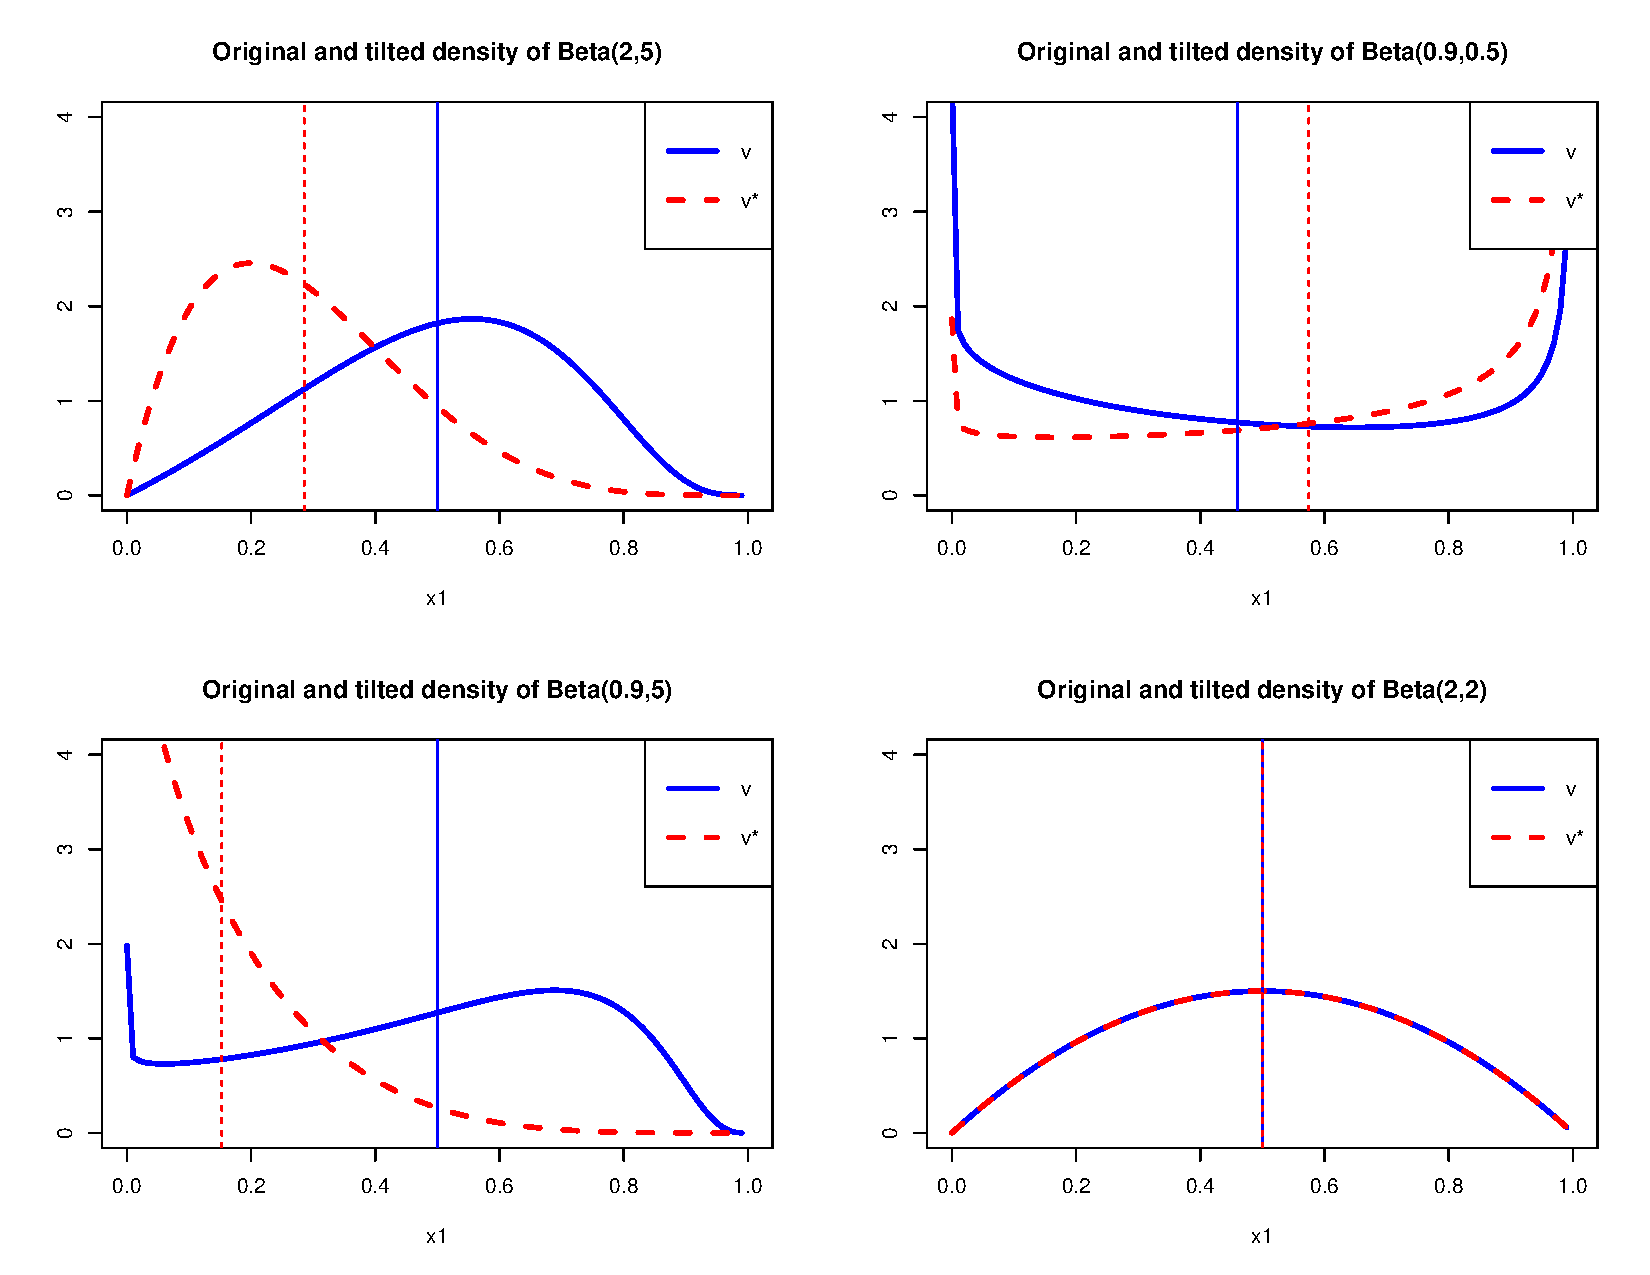
\includegraphics[width=\textwidth]{density_tilt.pdf}
\caption{Graphs of beta distributions for various shape parameters, before and after tilting. The vertical lines represent the means. As we can see, although the original densities have various means, the tilted densities all have mean 0.5, and when the original distribution already has the correct mean, it is not tilted.}
\label{fig:density_tilt}
\end{figure}

\subsubsection{Sampling from tilted density}
As we have seen in the proof of theorem 2, to construct the appropriate density $\nu$, we start with a density $\nu^*$, apply a change of variable to it, then tilt the result by diving it by $Dm^Tw$, which is bounded, in order to sample from the tilted density, we can sample from the original density $\nu^*$, transform the the samples, then apply the following Acceptance-Rejection step:

$$
U\leq m_{\min}/m^Tw
$$
where $m_{\min} = \min_d m_d$

This is because a realisation $W^*$ of $\nu^*$ that has been transformed has density $f$ and not $\nu$. But $m_{\min}/m^TW \leq 1$, so conditional on $W=w$ the event $U \leq m_{\min} /m^Tw$ has probability $m_{\min}/m^Tw$. Thus the marginal density of the $W$ for which the event occurs is proportional to $f(w)/(m^Tw)$ and has to be $\nu$.

The acceptance probability is given by
$$
\int \frac{m_{\min}}{m^Tw}f(w){\rm d}w = Dm_{\min} \int \nu (w) {\rm d} w = Dm_{\min}
$$

Thus the number of accepted samples is proportional to $m_{min}$, so the algorithm is the most efficient when all the $m_d$ are equal to $1/D$ which would mean our original density $\nu^*$ already satisfies the criteria and we would not have to run the algorithm at all.

\subsubsection{Tests}
Figure \ref{fig:historam_tilt} some examples of tilted mixtures of beta distributions, sampled using the algorithm, and the theoretical tilted distributions using the formula.

\begin{figure}[h]
\centering
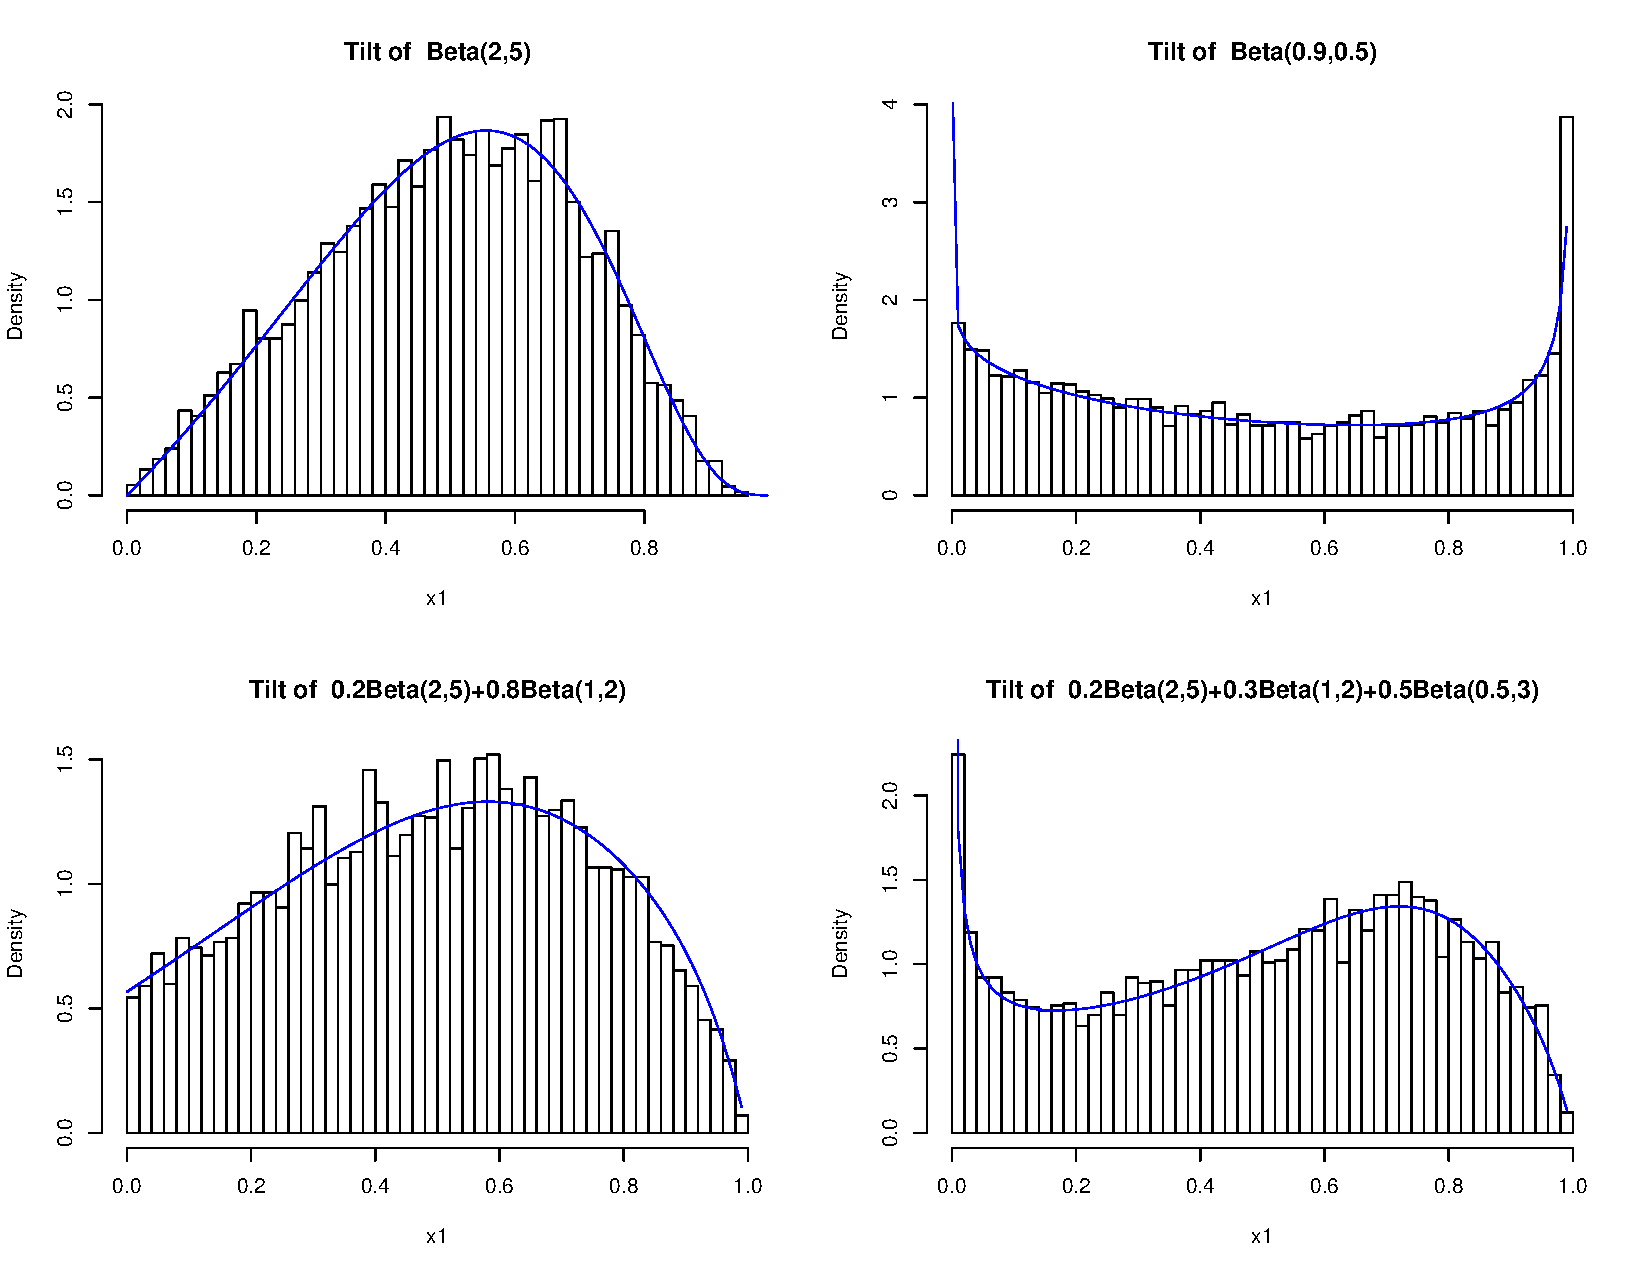
\includegraphics[width=\textwidth]{histogram_tilt.pdf}
\caption{Histograms of $10^4$ samples from various mixtures of beta distributions that have been tilted. The pdfs of the distributions are overlaid in blue. As we can see, the sampling algorithm for the tilted mixtures is correct.}
\label{fig:historam_tilt}
\end{figure}




\section{Tilted mixtures are dense}
%if possible, show that the class of tilted mixture distributions is dense in the class of distributions with mean 1/D (analogous to Appendix in Boldi and Davison)

\chapter{Statistical aspects}
\label{sec:stats}
\section{Likelihood fitting}
%likelihood fitting of the tilted distribution to data generated from the mixtures
%theory, explanation of how well the ML method works
%use of AIC/BIC to select numbers of components in the fitted mixture

We use the generic R optimiser \textit{optim} to minimise the negative log-likelihood function. In order to use it we first reparameterized the parameters, in order to express the $S_2$ constraint in a way that the optimiser can understand.

$$
\pi_k = \exp(\eta_k)/\left\{ 1+ \sum_{i=2}^K\exp(\eta_i)\right\}, \quad k=2,\ldots, K, 
$$
and 
$$
\pi_1 = 1/\left\{ 1+ \sum_{i=2}^K\exp(\eta_i)\right\}.
$$
We also reparametrize the $\alpha$ and $\beta$ parameters as

$$
\alpha_k = \exp(\xi_k), \quad \beta_k = \exp(\zeta_k), \quad k=1,\ldots,K,
$$

\begin{figure}[h]
\begin{tabular}{cccc}

	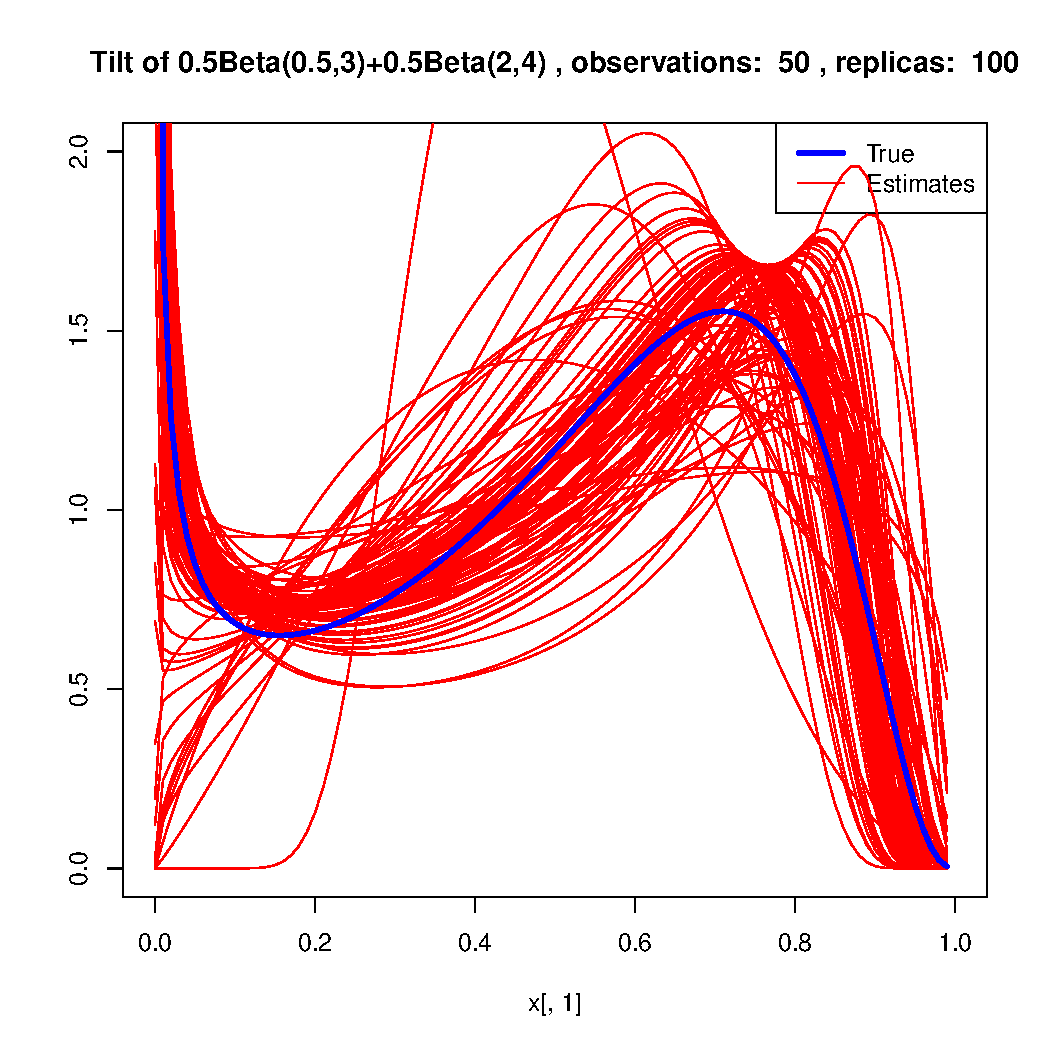
\includegraphics[width=\textwidth/4]{../img/p05_a05_b3_p05_a2_b4/tilted/K1/densities/n50_R100.pdf}
	&
	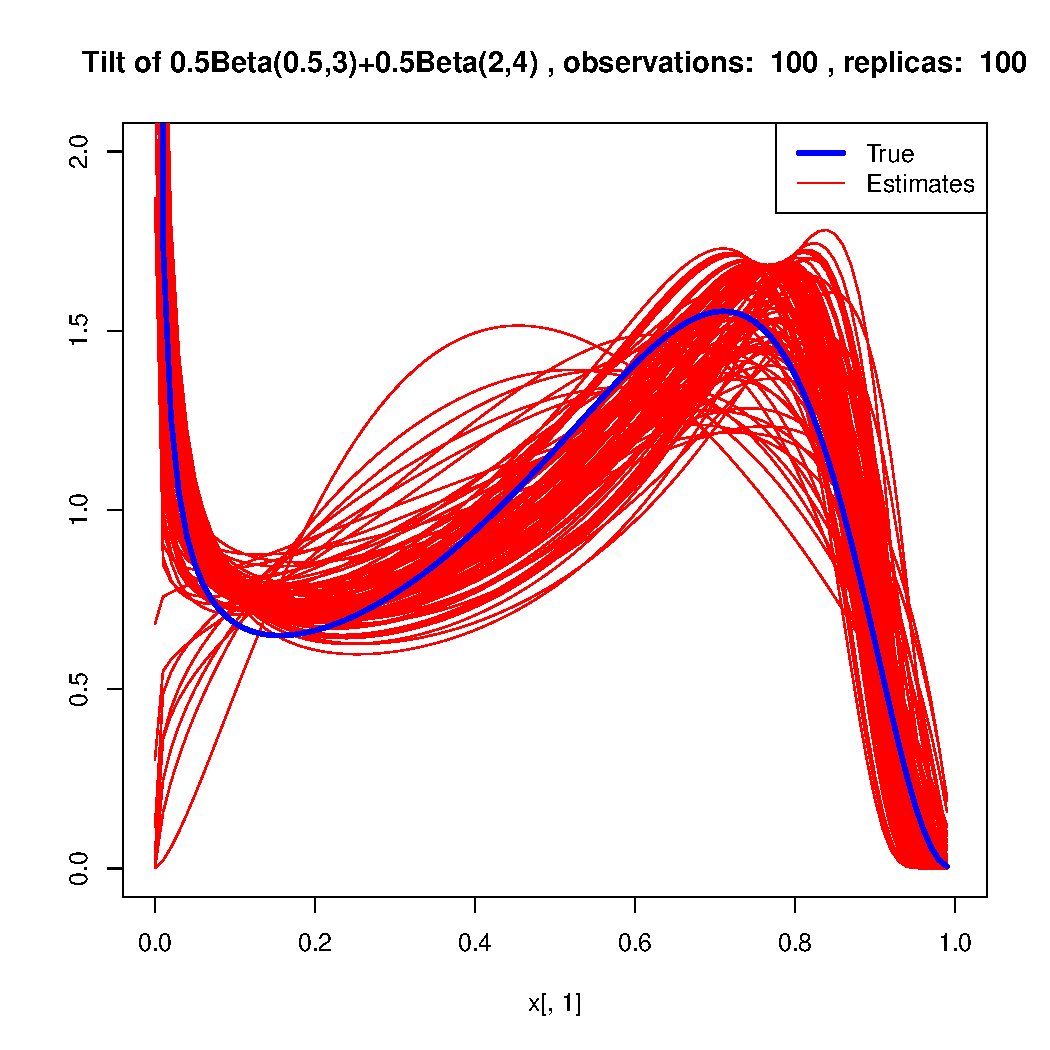
\includegraphics[width=\textwidth/4]{../img/p05_a05_b3_p05_a2_b4/tilted/K1/densities/n100_R100.pdf}
	&
	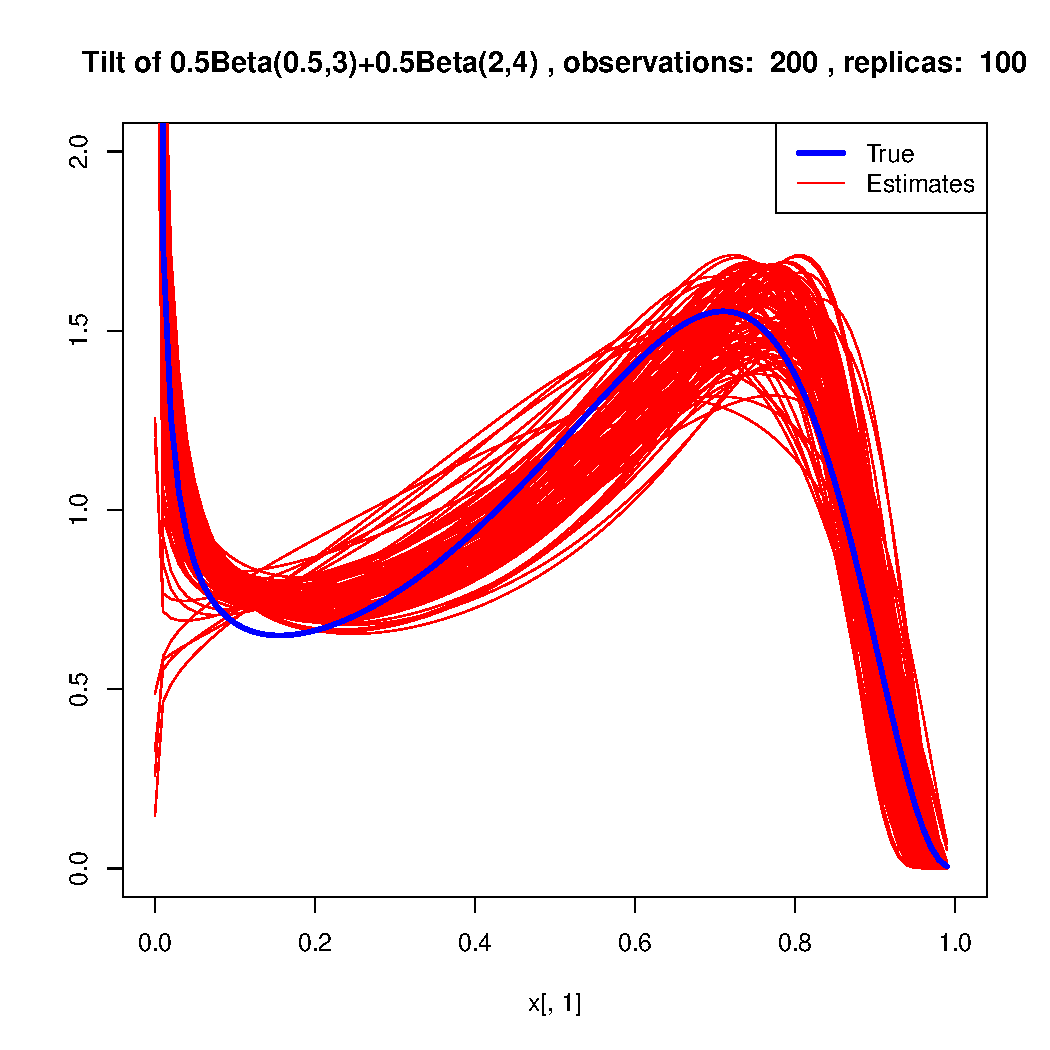
\includegraphics[width=\textwidth/4]{../img/p05_a05_b3_p05_a2_b4/tilted/K1/densities/n200_R100.pdf}
	&
	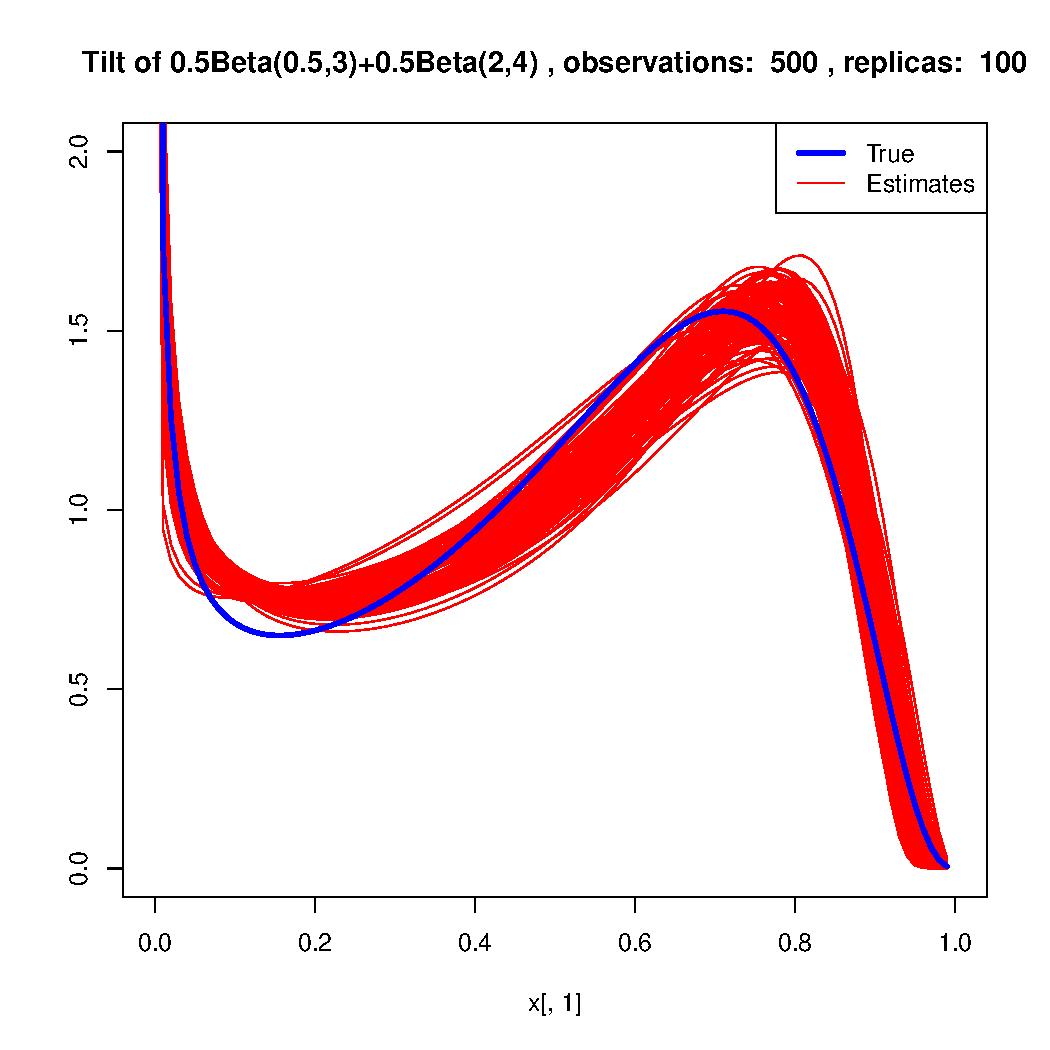
\includegraphics[width=\textwidth/4]{../img/p05_a05_b3_p05_a2_b4/tilted/K1/densities/n500_R100.pdf}\\
	
	
	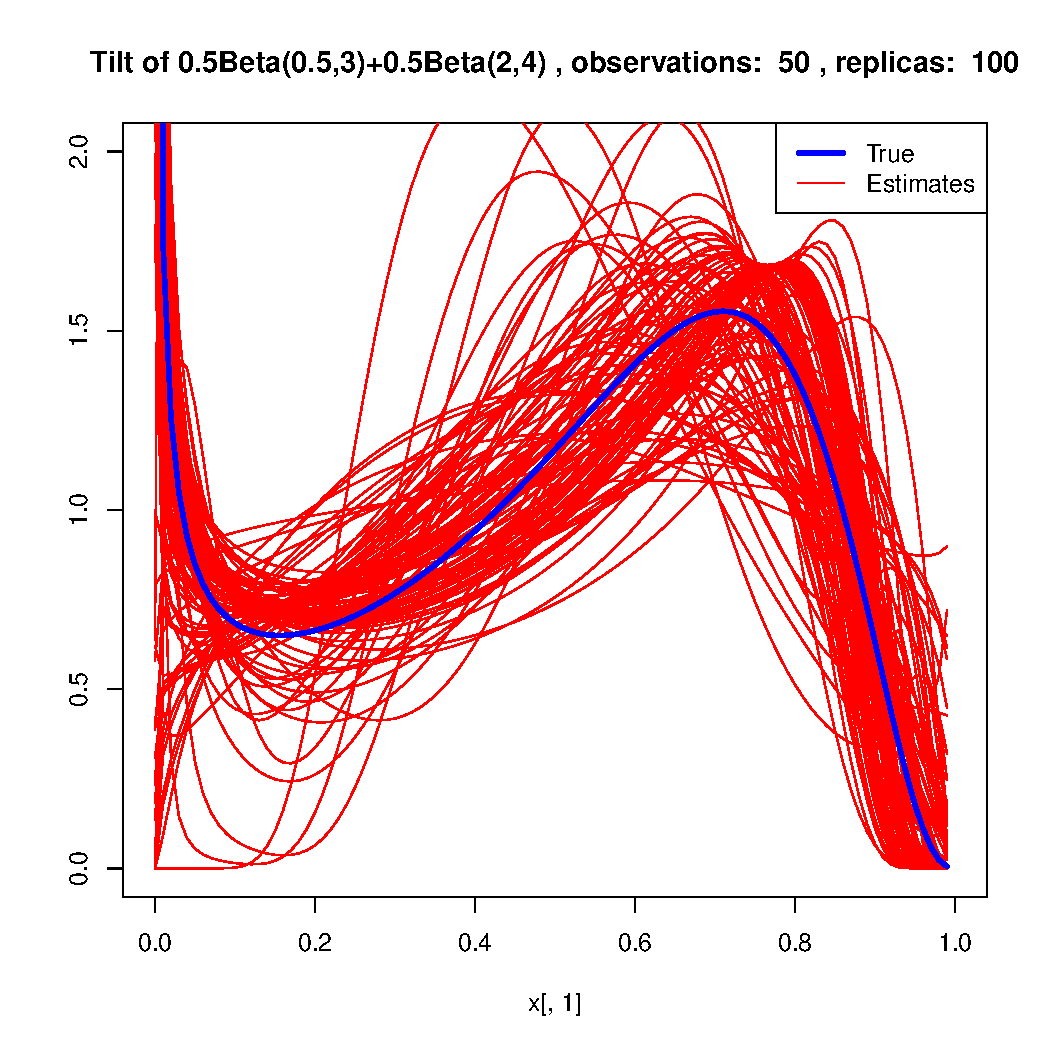
\includegraphics[width=\textwidth/4]{../img/p05_a05_b3_p05_a2_b4/tilted/K2/densities/n50_R100.pdf}
	&
	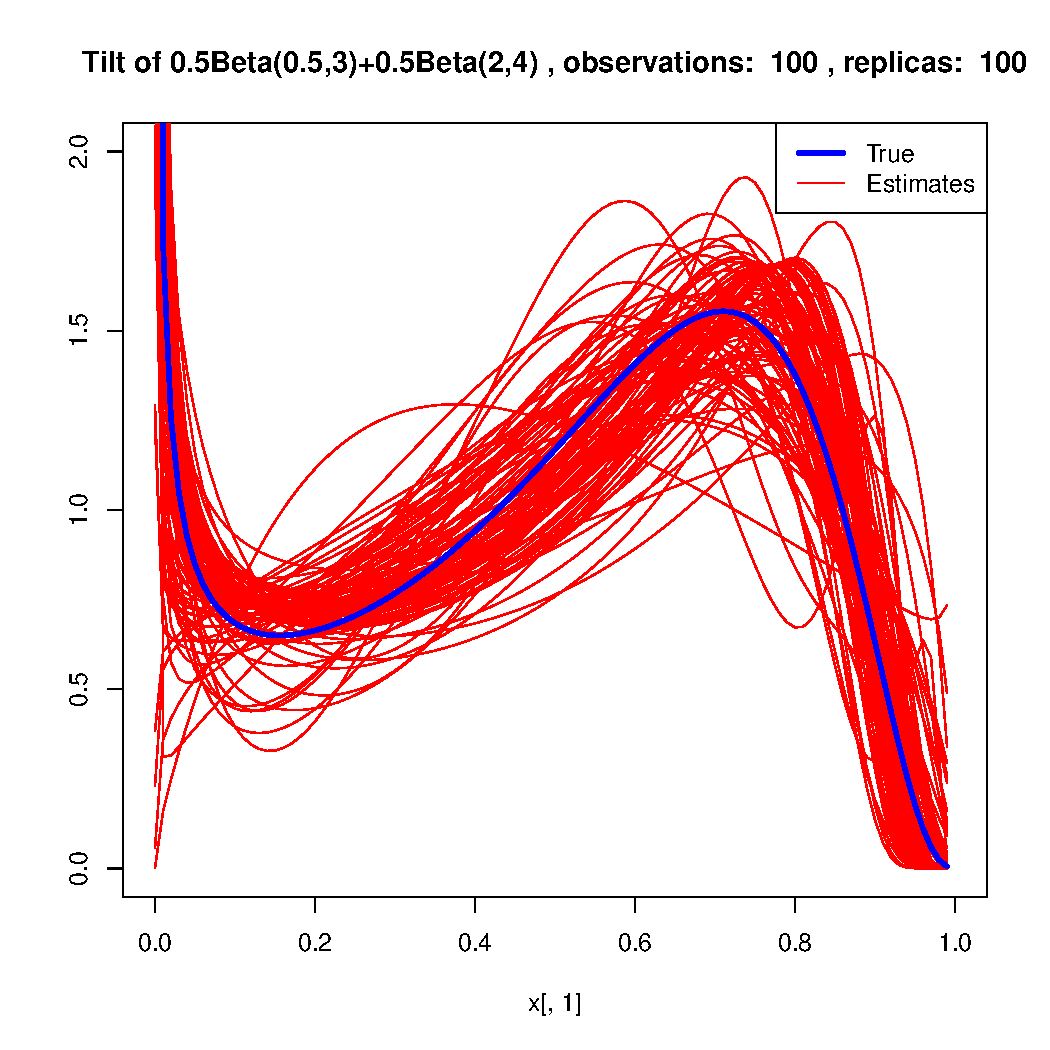
\includegraphics[width=\textwidth/4]{../img/p05_a05_b3_p05_a2_b4/tilted/K2/densities/n100_R100.pdf}
	&
	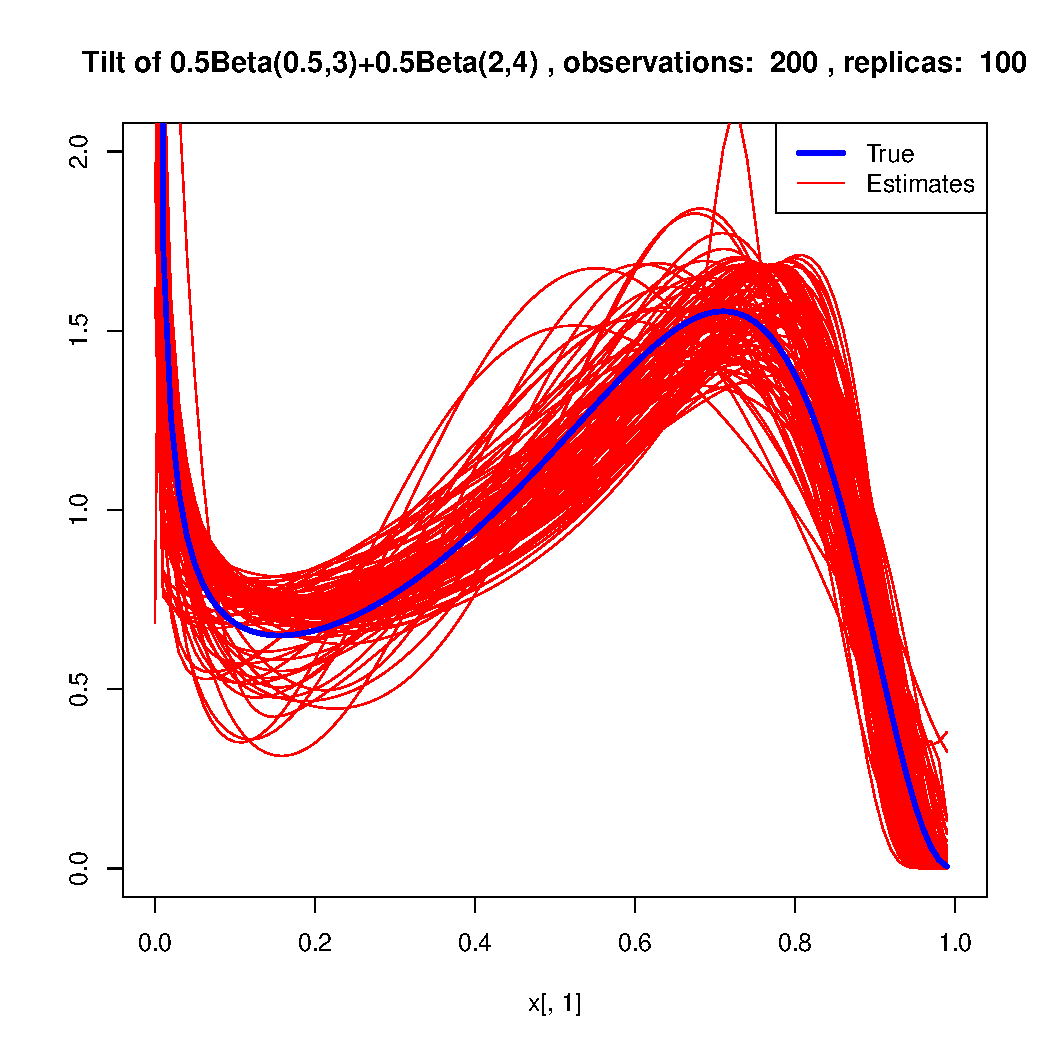
\includegraphics[width=\textwidth/4]{../img/p05_a05_b3_p05_a2_b4/tilted/K2/densities/n200_R100.pdf}
	&
	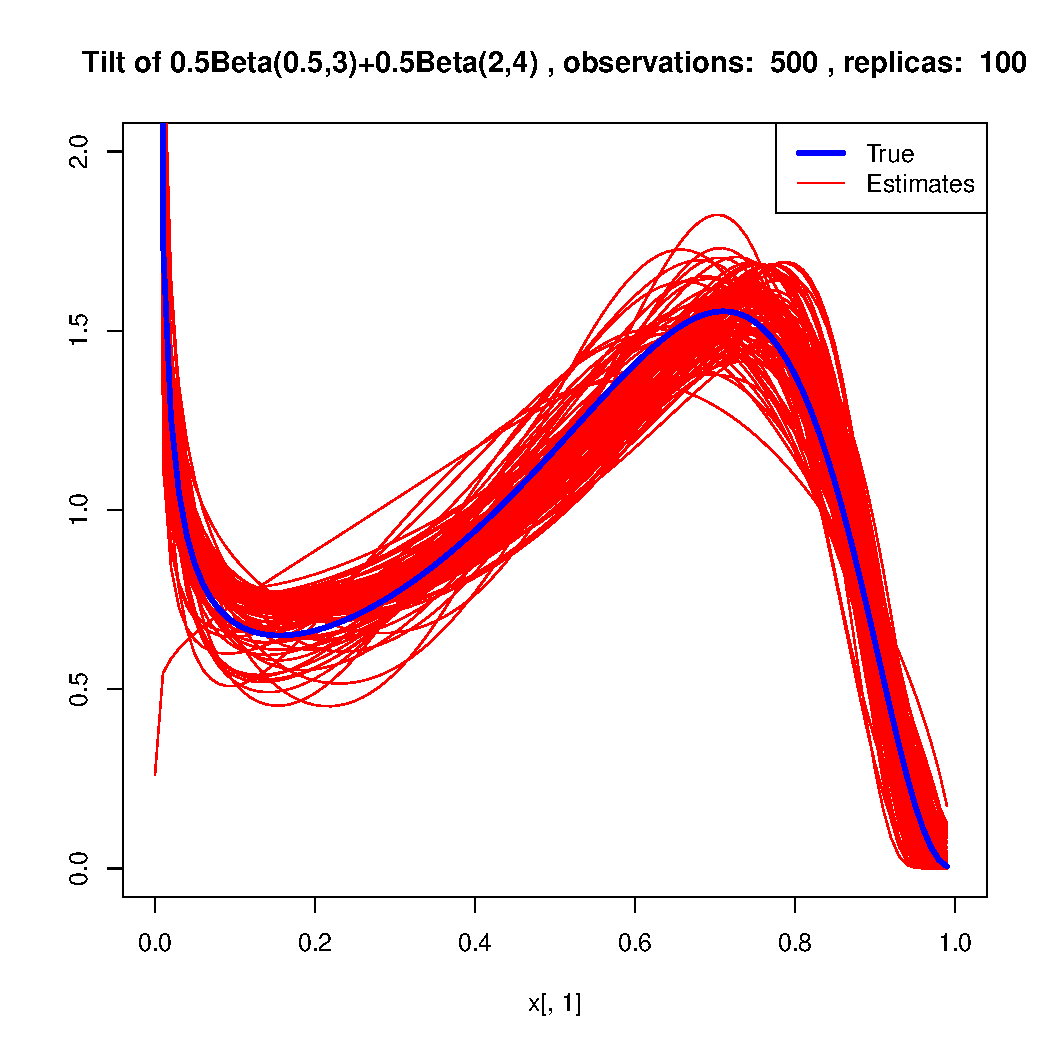
\includegraphics[width=\textwidth/4]{../img/p05_a05_b3_p05_a2_b4/tilted/K2/densities/n500_R100.pdf}\\
	
	
	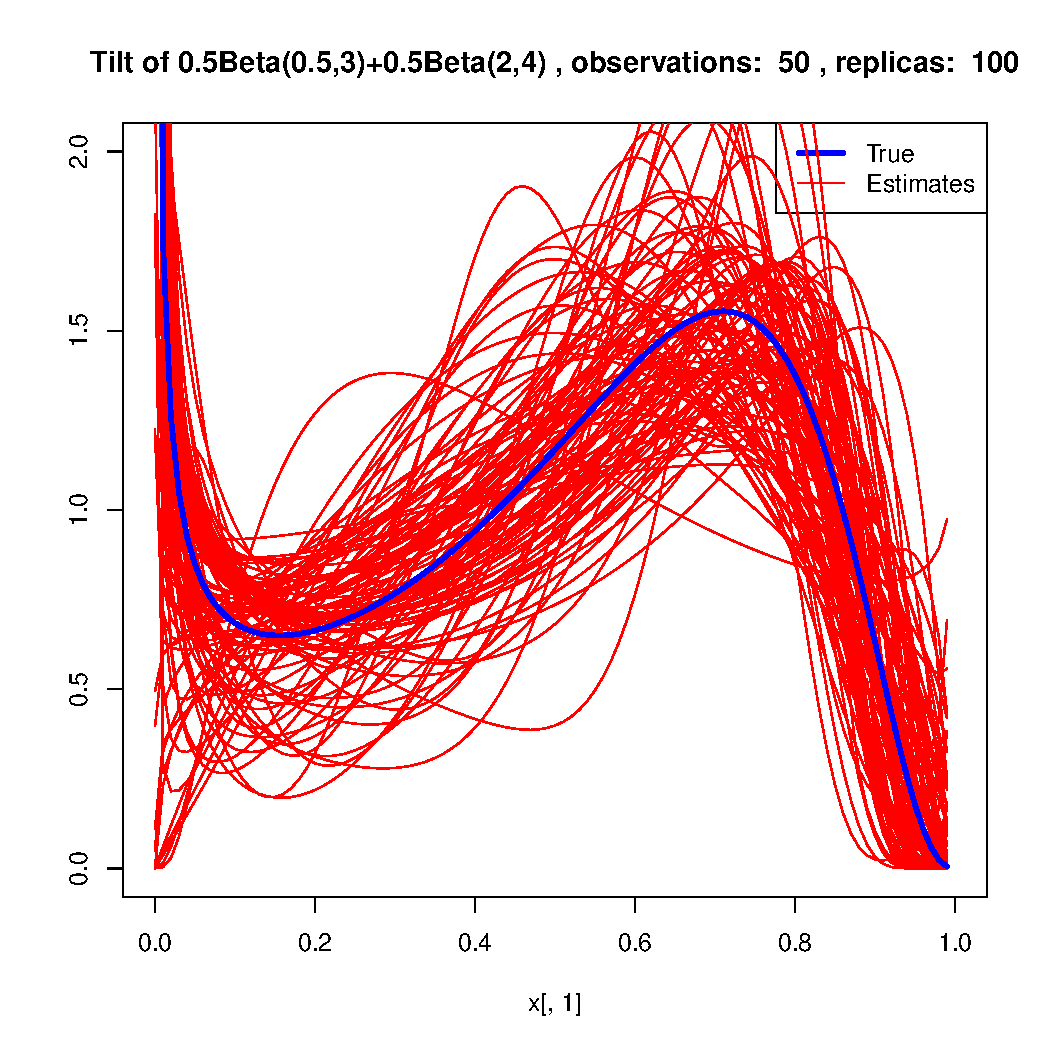
\includegraphics[width=\textwidth/4]{../img/p05_a05_b3_p05_a2_b4/tilted/K3/densities/n50_R100.pdf}
	&
	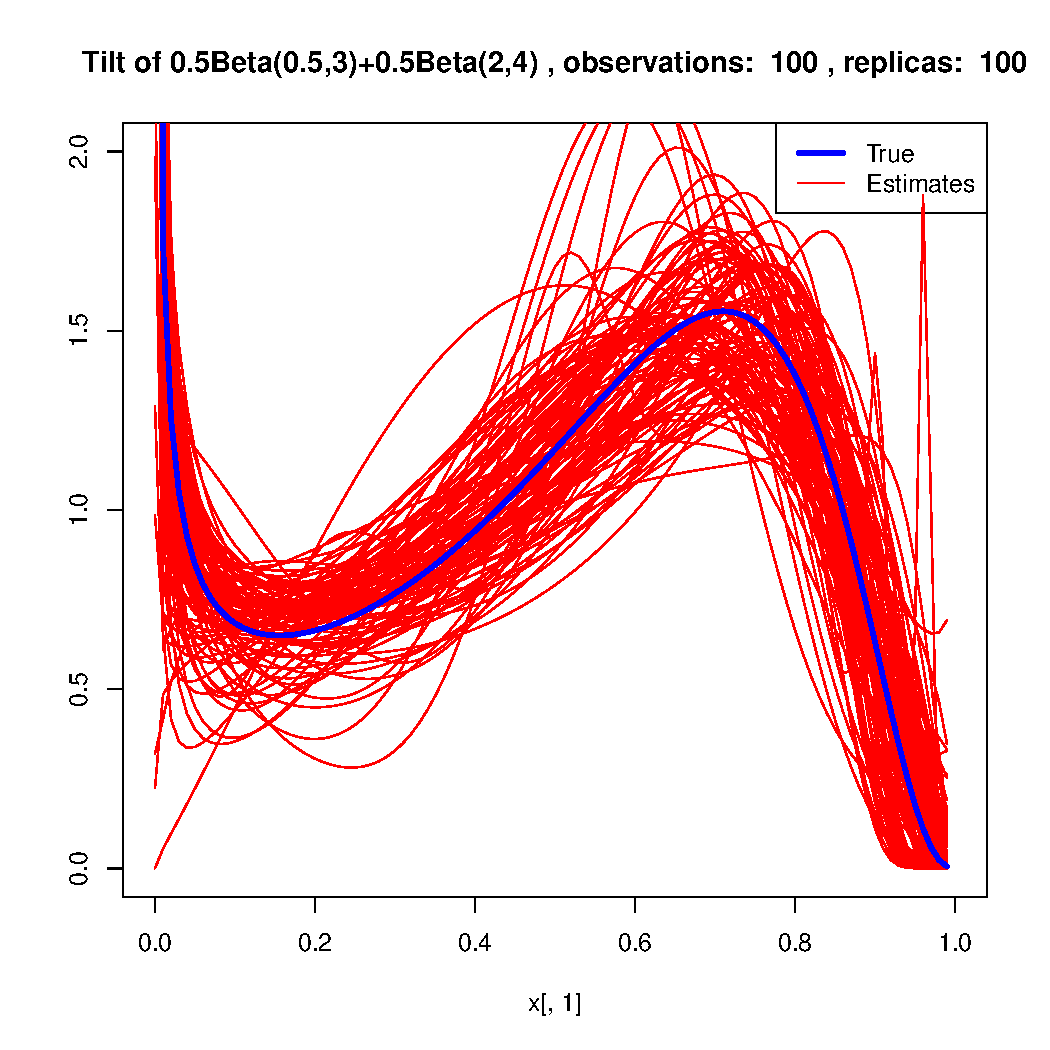
\includegraphics[width=\textwidth/4]{../img/p05_a05_b3_p05_a2_b4/tilted/K3/densities/n100_R100.pdf}
	&
	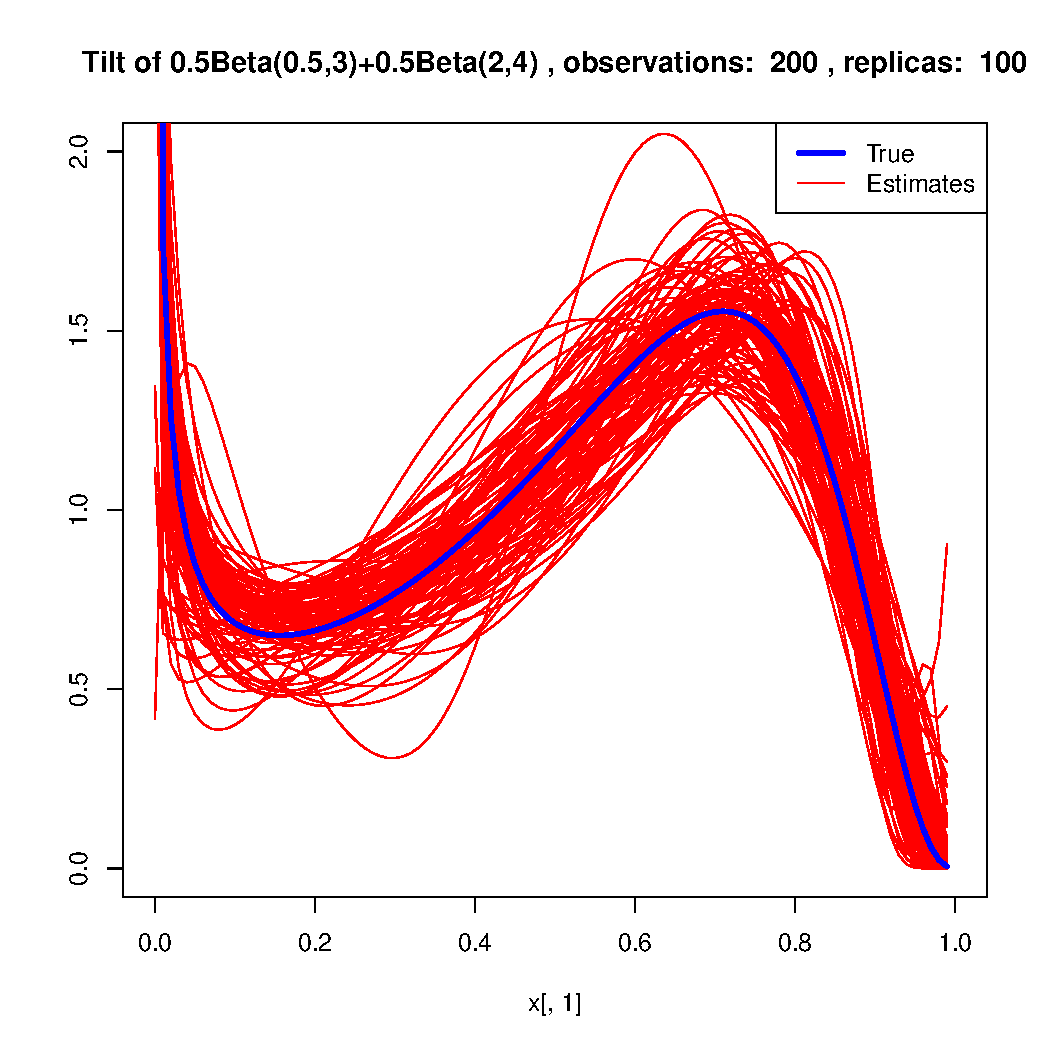
\includegraphics[width=\textwidth/4]{../img/p05_a05_b3_p05_a2_b4/tilted/K3/densities/n200_R100.pdf}
	&
	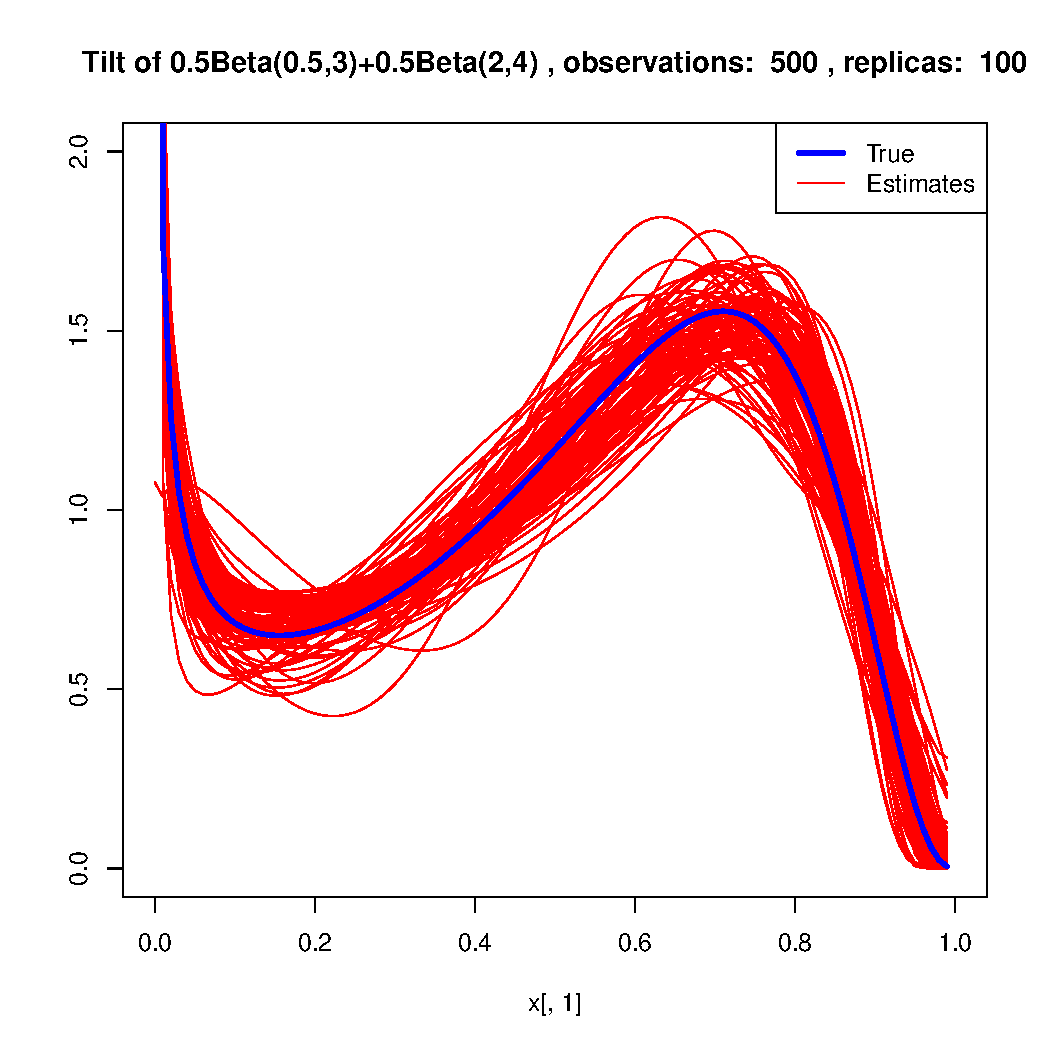
\includegraphics[width=\textwidth/4]{../img/p05_a05_b3_p05_a2_b4/tilted/K3/densities/n500_R100.pdf}\\
	
\end{tabular}
\caption{MLE fits to samples of size, from left to right, $n=50$, $n=100$, $n=200$ and $n=500$, with different number of betas in the mixture. From top to bottom: $K=1$, $K=2$ (which is the number that generated the data), and $K=3$, using a \textit{Nelder-Mead} optimiser each time, with a maximum of 500 iterations.}
\label{fig:TDB1}
\end{figure}

\begin{figure}[h]
\begin{tabular}{cc}
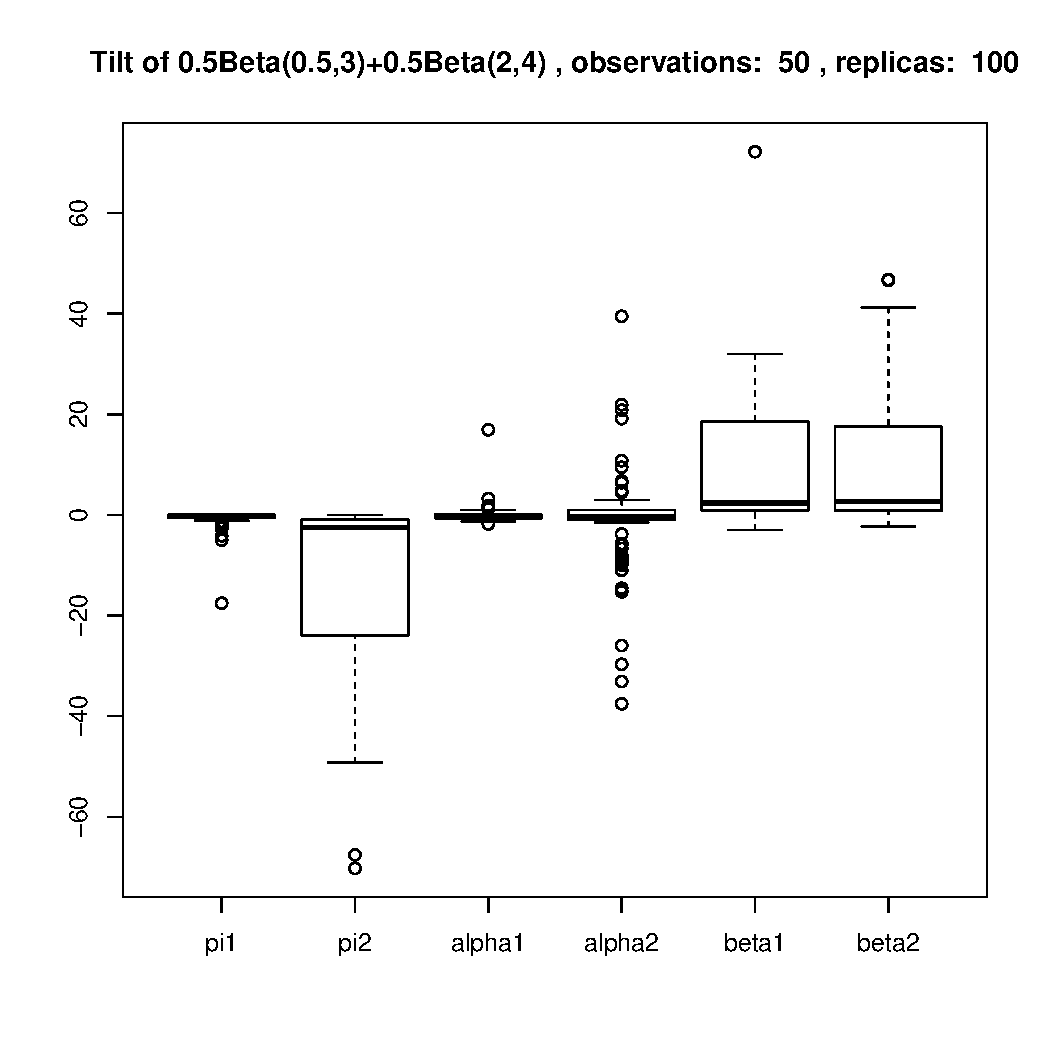
\includegraphics[width=\textwidth/2]{../img/p05_a05_b3_p05_a2_b4/tilted/K2/bxplots/n50_R100.pdf}
&
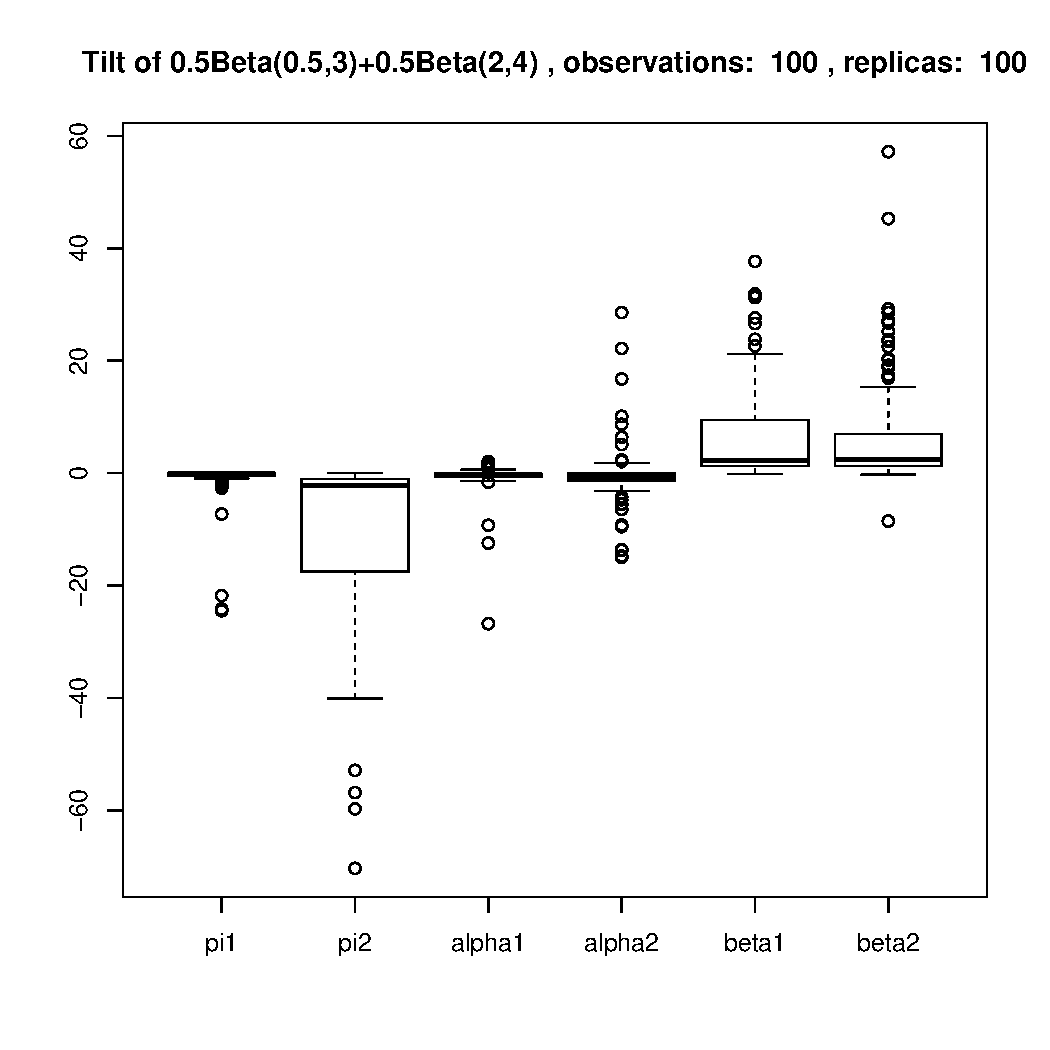
\includegraphics[width=\textwidth/2]{../img/p05_a05_b3_p05_a2_b4/tilted/K2/bxplots/n100_R100.pdf}\\

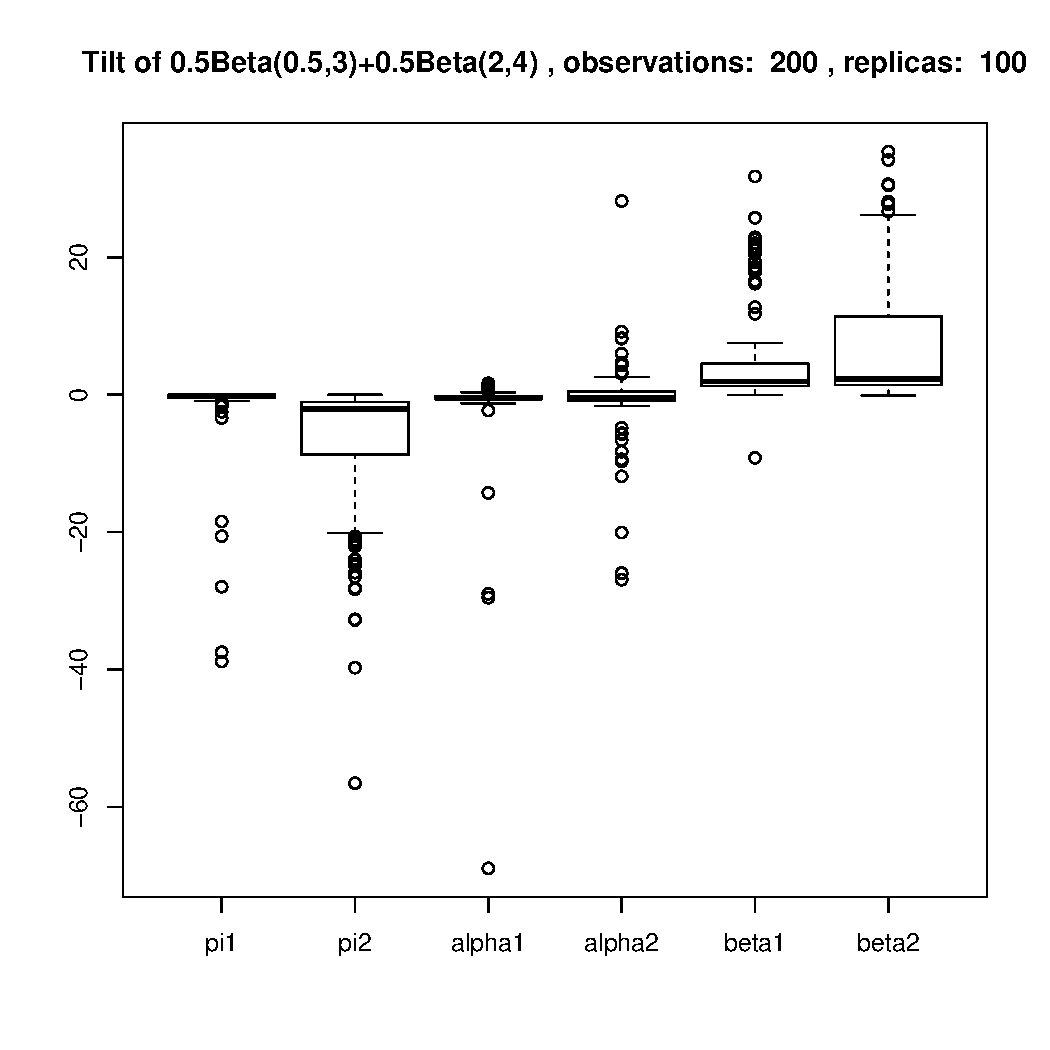
\includegraphics[width=\textwidth/2]{../img/p05_a05_b3_p05_a2_b4/tilted/K2/bxplots/n200_R100.pdf}
&
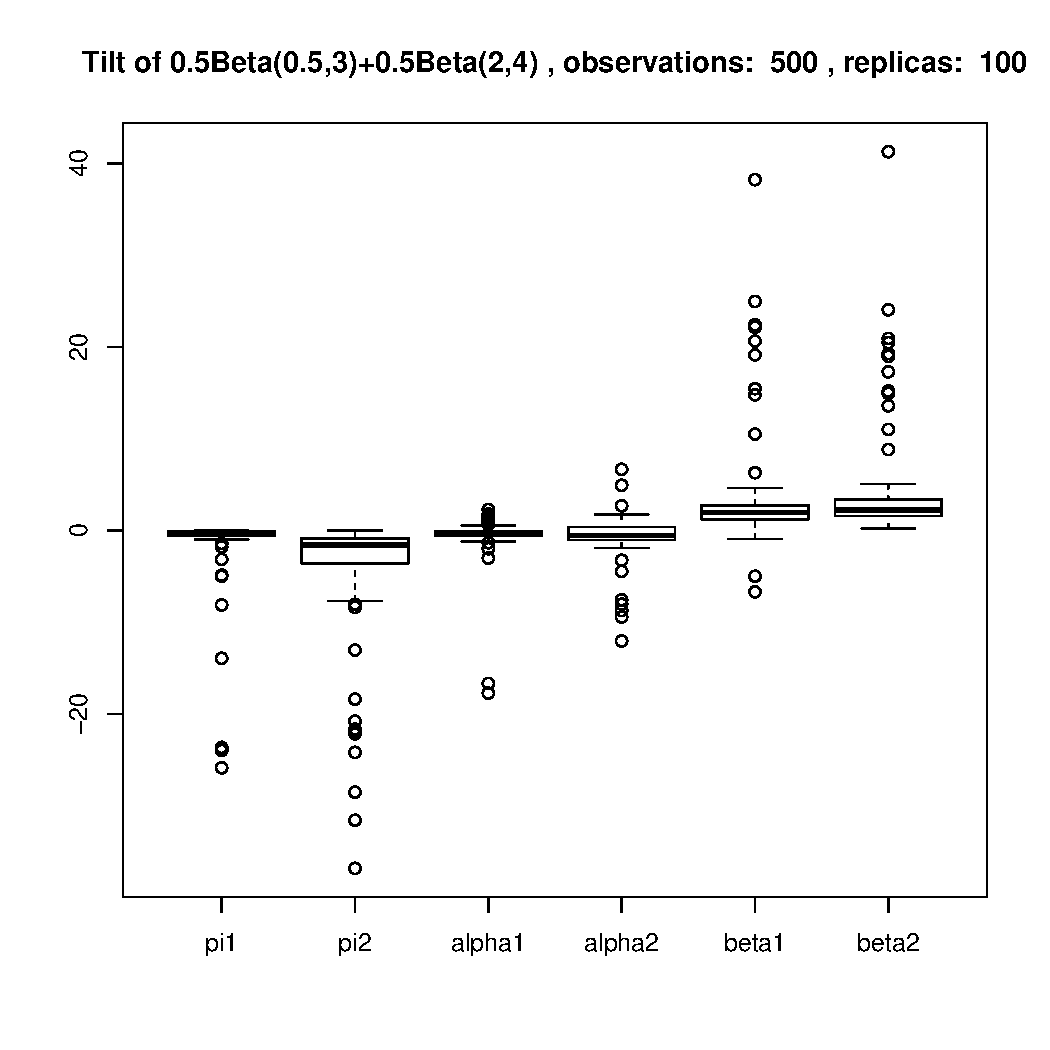
\includegraphics[width=\textwidth/2]{../img/p05_a05_b3_p05_a2_b4/tilted/K2/bxplots/n500_R100.pdf}\\
\end{tabular}
\caption{Boxplot of log MLE estimates (Nelder-Mead, maxit 500), for $K=2$ and sample of 50, 100, 200, 500 observations}
\label{fig:TBD2}
\end{figure}


\begin{figure}[h]
\centering
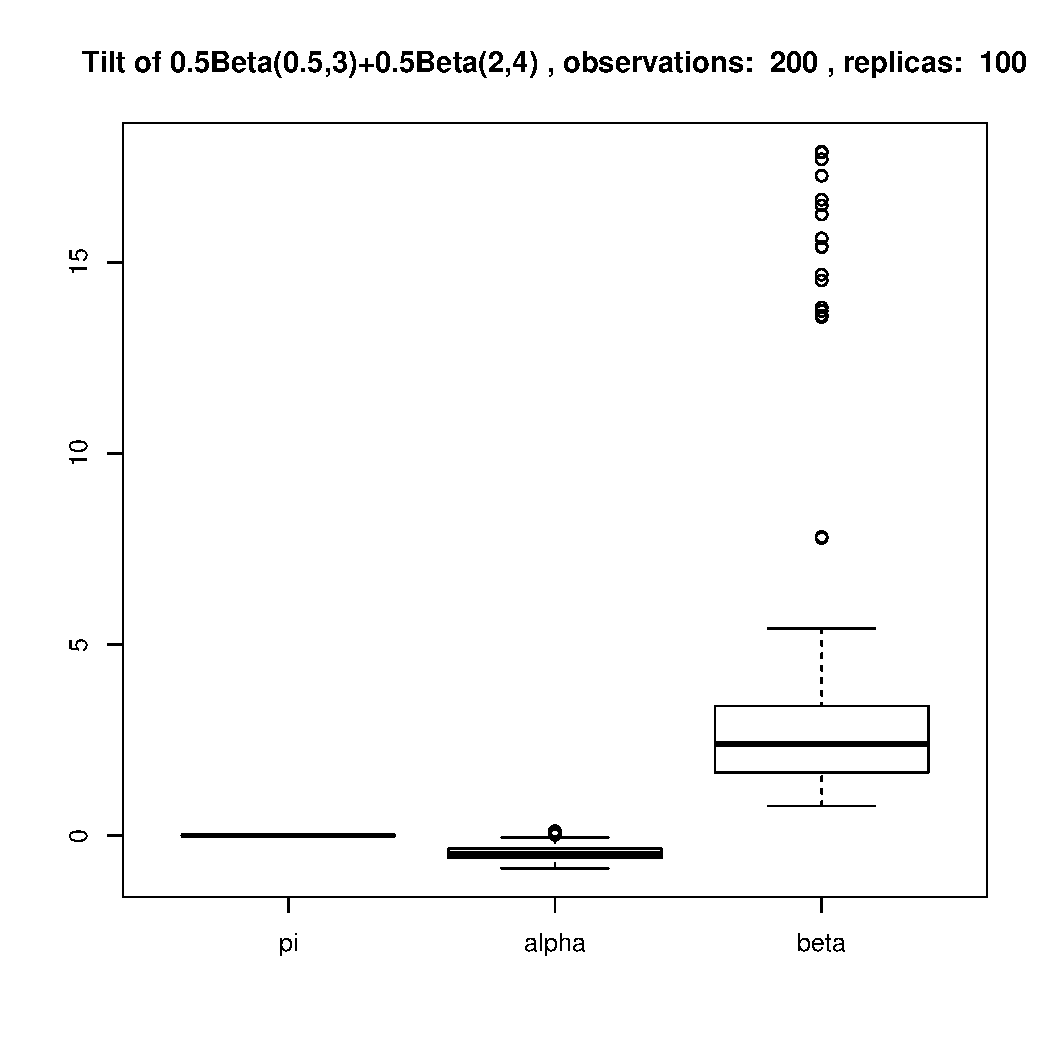
\includegraphics[width=\textwidth]{../img/p05_a05_b3_p05_a2_b4/tilted/K1/bxplots/n200_R100.pdf}
\caption{Boxplot of log MLE estimates (Nelder-Mead, maxit 500), for $K=1$ and sample of 200 observations}
\label{fig:TBD6}
\end{figure}

\begin{figure}[h]
\centering
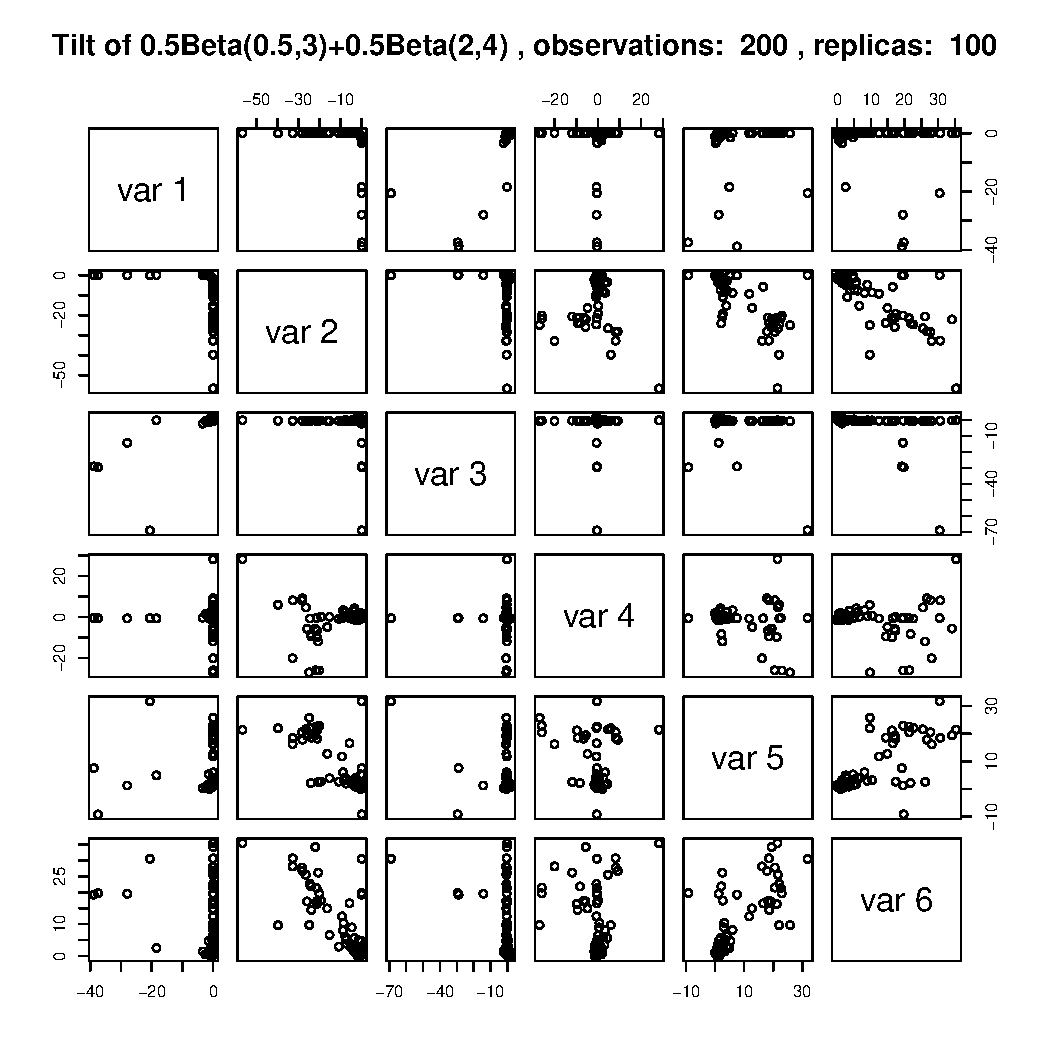
\includegraphics[width=\textwidth]{../img/p05_a05_b3_p05_a2_b4/tilted/K2/pairs/n200_R100.pdf}
\caption{pairs plot of log MLE estimates (Nelder-Mead, maxit 500), for $K=2$ and sample of 200 observations}
\label{fig:TBD7}
\end{figure}

\noindent
to ensure that the parameters can take any values in $\mathbb{R}$. There are $3K-1$ parameters to estimate, which can then be transformed back into the original parameterization after estimation. Initially, we consider $K$ to be a fixed parameter, and for given data we will try to fit with various values of $K$, including the real value, to see the accuracy, and if values of $K$ that are close, but not correct give a ``good enough" estimation (for example we could use a smaller $K$ than the true $K$ and still have a model that is accurate ``enough" for certain purposes. Then we shall try to consider $K$ as a parameter to be estimated as well, using methods such as step-AIC/BIC to select the model.

\section{Numerical experiments}
%Box plots of estimates and some measure of error (e.g. integrated squared error ? Hellinger distance ?) when (a) true distribution is fitted to the data; (b) data are simulated from some other distribution (i.e. not a mixture)
%for (say) n=50, n=100, n=200, n=500, each with maybe 100, maybe 200 replicates ?



As a measure of the error between the true density $f$ and the estimated density based on n samples $f_n$, we will use the integrated square error, defined as

$$
{\rm err}(f_n) := ||f_n - f||^2_2 = \int_0^1(f_n(x)-f(x))^2dx
$$

In Section \ref{sec:truedist} we fitted a tilted beta mixture to data actually simulated from a tilted beta mixture, then in Section \ref{sec:wrongdist} we fitted a tilted beta mixture to data simulated from other distributions (i.e., not from a beta mixture).

For each test distribution, we simulate $R=100$ samples of $n=50$, $n=100$, $n=200$, and $n=500$ independent observations. The Maximum Likelihood Estimation is done with ten different sets of initial parameters chosen uniformly at random between $-0.5$ and $+0.5$.

\subsection{Data simulated from mixture}
\label{sec:truedist}

First we generated data using a tilted mix of two beta distributions, $0.5Beta(0.5,3) + 0.5Beta(2,4)$, to test how well the maximum likelihood estimation would work. In Figure \ref{fig:TDB1} we see that for samples with a high number of observations, even estimating with a different number $K$ of components, the results are good, which suggests that we could indeed use a step-AIC/BIC method, starting with a single tilted beta distribution, and keep estimating with more until the added accuracy is no longer significant. Looking at the case n=50, however, we see a lot of volatility and artefacts. Some of the estimations have clearly not converged in 500 iterations of the Nelder-Mead algorithm, even when the correct number $K$ of betas is used.
\\

Looking at the boxplots of the log parameter for $K=2$, (Figure \ref{fig:TBD2}) we see that there are a lot of very large and very small values. This makes the analysis of the boxplots difficult. But looking at Figure \ref{fig:TDB1} we can guess what is happening: as the algorithm fits relatively well with just just a single beta distribution instead of two, all the cases with a very small $\pi_i$, is just the algorithm fitting one of the components very well, which sends the other component to insignificance. As for very small/large values for $\alpha_i$ and $\beta_i$, our hypothesis is that in the cases where the algorithm fitted one component really well, and the other component can take pretty much any value it wants, as it's contribution to the mixture has hardly any weight.
\\

To try to confirm this, first we can look at a boxplot of one of the fits with $K=1$, and indeed if we look at Figure \ref{fig:TBD6} we do see that the parameters seem a lot better contained. The group of $\beta$ outliers could be explained by the fact the original density we are working with increases asymptotically on the left side (the side controlled by the $\alpha$ parameters) so the relative importance of the right side (controlled by the $\beta$ parameter) might be low. 
\\

Another check we can do is have a look at a pairs plot for $K=2$, to see if low values of $\pi_i$ correspond to very small/large values of $\alpha_i$ and $\beta_i$. In Figure \ref{fig:TBD7}, we have the pairs plot for $n=200$ samples. Comparing Var2 (a $\pi_i$) vs Var6 (the corresponding $\beta_i$), we clearly see a clump down at the right corner, where stuff is happening according to plan, but also that as the weight of the component gets smaller, the value of the $\beta$ parameter gets larger and more volatile. If we look at Var2 vs Var4 (the corresponding $\alpha_i$), we also see a nice clump around $0$ on the right side, where the weight of the component is still significant, and as the weight gets smaller, the $\alpha$ parameter gets more volatile, with a slight tendency for very small values.
\\


To try and fight this phenomenon, we will try two things: the first is to use a constrained optimiser (L-BFGS-B) to keep all the log-parameters in a box of say, +/- 5, and the second is to first fit with a single component, and use those estimates, along with added random ones, as a starting point for a round of Nelder-Mead or BFGS (though, considering that the problem seems to be that the algorithms are overfitting one component in neglect of the other, this probably won't help, and method 1 might be the only course of action.)

\subsection{Data simulated from other distributions}
\label{sec:wrongdist}

\section{Numerical experiments}
Much as in the previous section, we have fitted tilted beta mixtures to various simulated data, but this time we also estimate the marginal parameters.

\section{Numerical example}
%Fitting the mixture to some (standard?) datasets to see how many components are needed, asses the quality of the fit, etc.

\subsection{The data}
The data we will be exploring consists of 2 variables, daily maximum windspeed (mph) and the Fosberg fire weather index FFWI, for 20 locations in Southern California. The FFWI is an index to give some measure of the potential influence of the weather on wildland fires. It is calculated using temperature, relative humidity and windspeed, and calibrated to equal 100 when the windspeed is 30 mph and the air moisture content is 0. Any value of FFWI higher than 100 is rounded down to 100.
The data originated from the Hadley Centre (\url{https://www.metoffice.gov.uk/hadobs/hadisd/}) and were processed by Professor Ben Shaby to get them into the form they are now. Notably, the data went under some corrections for bad data, windspeed conversion from m/s to mph, calculation of the FFWI and they may have been homogenised to deal with instrument drift and other issues. The windspeed values may therefore be seem a bit odd, and to get windspeeds in m/s again, the windspeed would need to be divided by $2.23694$.
The processed data is available on Github (\url{https://github.com/Sekarski/MasterSemestreProject/data/had_ffwi_wind-SantaAna.RData}).

For this project we have chosen the 3 locations out of the 20 that have the most data point to study. These are locations 1,17 and 15, with respectively 15'400, 15'399 and 15'372 points, after removing missing or incomplete data points.

\subsection{Making the data angular}

\begin{figure}[h]
\begin{tabular}{ccc}
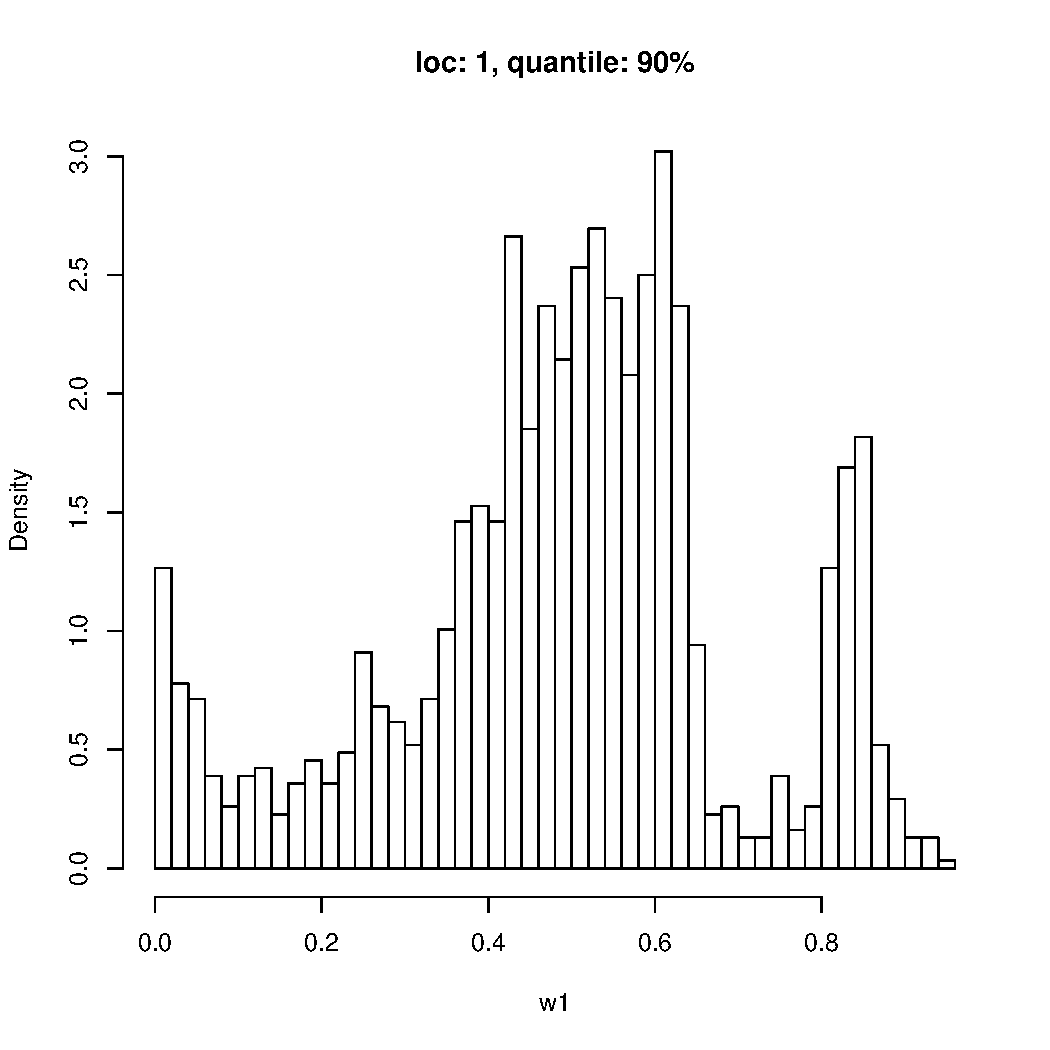
\includegraphics[width=\textwidth/3]{../img/loc1/quantile90/histogram.pdf}
&
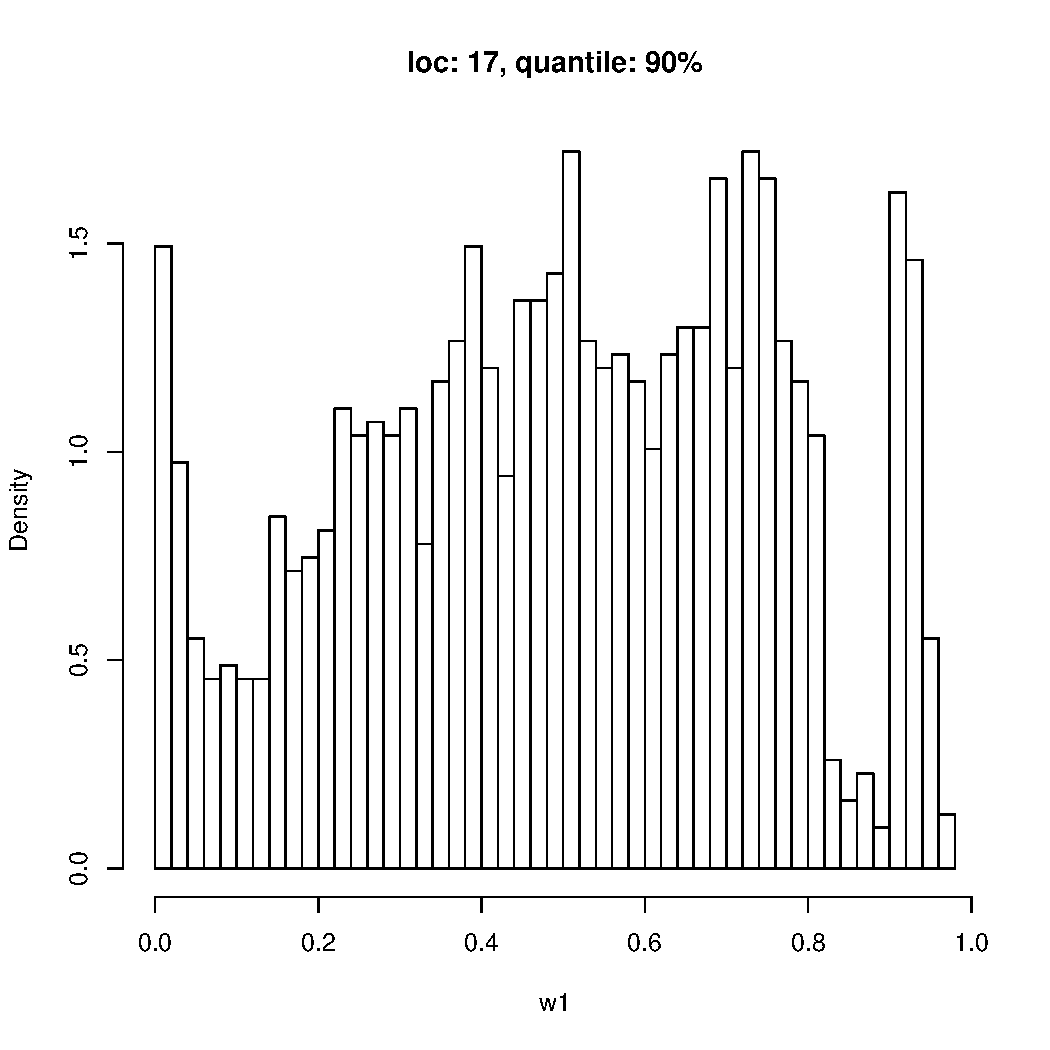
\includegraphics[width=\textwidth/3]{../img/loc17/quantile90/histogram.pdf}
&
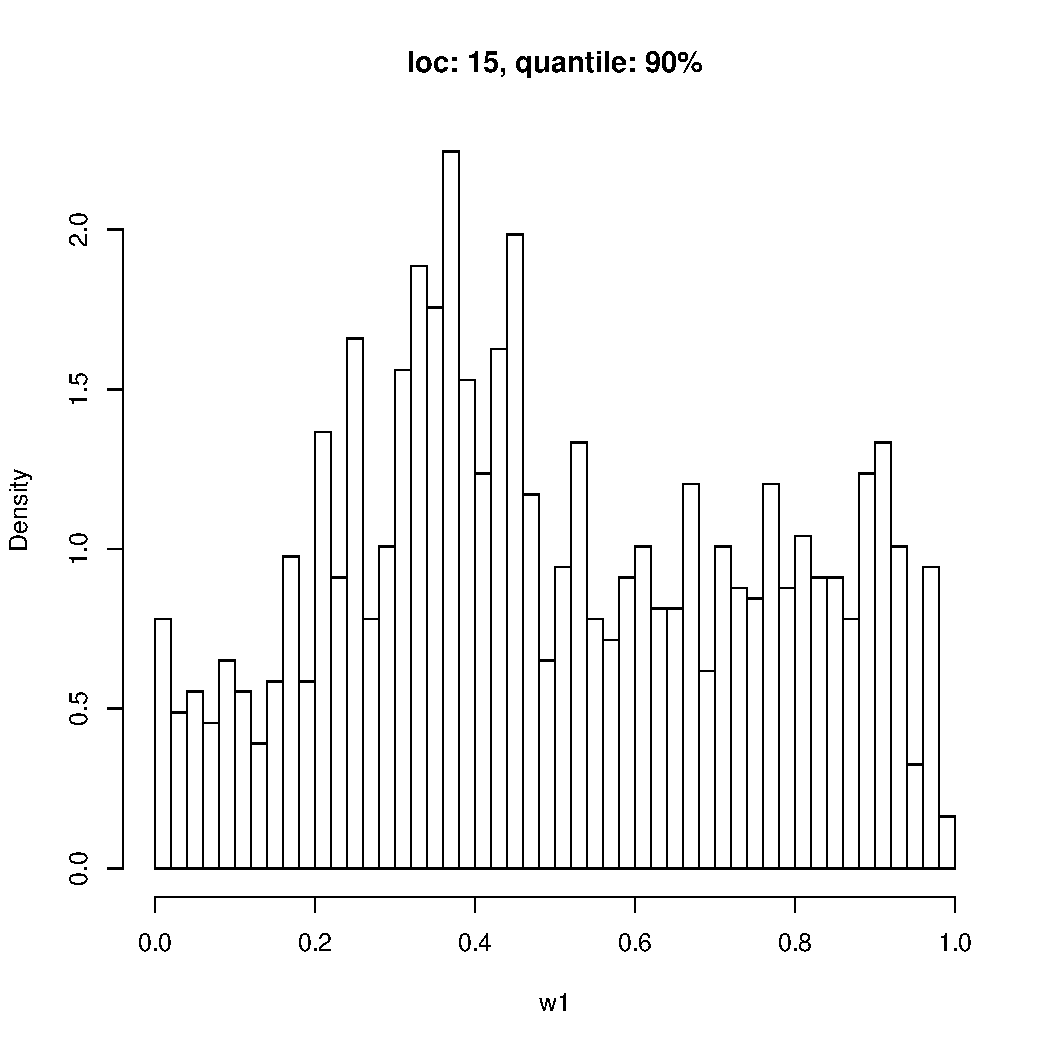
\includegraphics[width=\textwidth/3]{../img/loc15/quantile90/histogram.pdf}\\
\end{tabular}
\caption{Histograms for the angular data above the 90\% quantile for locations 1,17 and 15 respectively.}
\label{fig:data_hist}
\end{figure}

In order to fit our tilted mixtures, we first need to make the data angular.
Let $X=(X_1,X_2)$ be the bivariate data at one of the locations, and $X_i = (x_{i1}, \ldots, x_{in})$ for $i=1,2$.
We start by fitting a Generalized Pareto Distribution to the exceedances over thresholds $u_i$ on each margins. For the thresholds, we chose the 90\% quantiles for each margin. We get estimates $\hat \sigma_i$ and $\hat \xi_i$  and fitted distributions
$$
\hat F_i(x) = n^{-1} \sum_{j=1}^n {\rm I}_{\{x_{ij}\leq x\}} (x)  {\rm I}_{\{x\leq u_i\}} (x) + \left[ 1 - \frac{n_{u_i}}{n} \times \left\{1 + \hat\xi_i\frac{(x-u_i)}{\hat \sigma_i} \right\}^{-1/\hat\xi_i}_+ \right] {\rm I}_{\{x>u_i\}} (x),
$$
Were $n_{u_i}$ is the number of observations above the threshold $u_i$. We then apply the transformation $ Z_i = -1/ \log \hat F_i(X_i)$ to bring $X$ to the unit Fréchet scale, then tilt the data by setting
$$
W_i = Z_i/(Z_1 + Z_2), \quad i=1,2.
$$
Finally, we get the data on which we will do the fitting by selecting all the observation where $z_1j + z_2j$ are above the 90\% quantile of $Z_1 + Z_2$. That is:
$$
W = \{ (w_{1j},w_{2j}) : z_{1j} + z_{2j} > r_{90} \}
$$
Where $r_{90}$ is the 90\% quantile. Figure \ref{fig:data_hist} show what the distribution of $W_1$ looks like. All three locations have different shapes.


\subsection{Fitting}
%K1 loc1 fit AIC: -458.409057486619 1 1.15 5.83
%K2 loc1 fit AIC: -711.67001541868 0.9356 15.42  2.402 0.644 0.911 0.952
%K3 loc1 fit AIC: -705.333755225558 0.9456 13.672 2.41 0.0258 0.893 3.5 0.0286 2.547 2.53
%K1 loc17 fit AIC: -147.172809890411 1 0.88 2.41
%K2 loc17 fit AIC: -194.223475679536  0.9348 2.17 1.68 0.0652 0.666 14.01
%K3 loc17 fit AIC: -185.575120747714 0.172 0.567 0.988 0.713 3.065 1.678 0.115 4.122 1.546
%K1 loc15 fit AIC: -79.956280458566 1 1.4 1.29
%K2 loc15 fit AIC: -116.805491118043 0.0665 1.26 0.667 0.9335 8.22 0.974
%K3 loc15 fit AIC: -110.70470605339 0.9123 5.17 1.012 0.715 2.13 0.946 0.162 1.48 7.625


\begin{figure}[h]
\begin{tabular}{ccc}
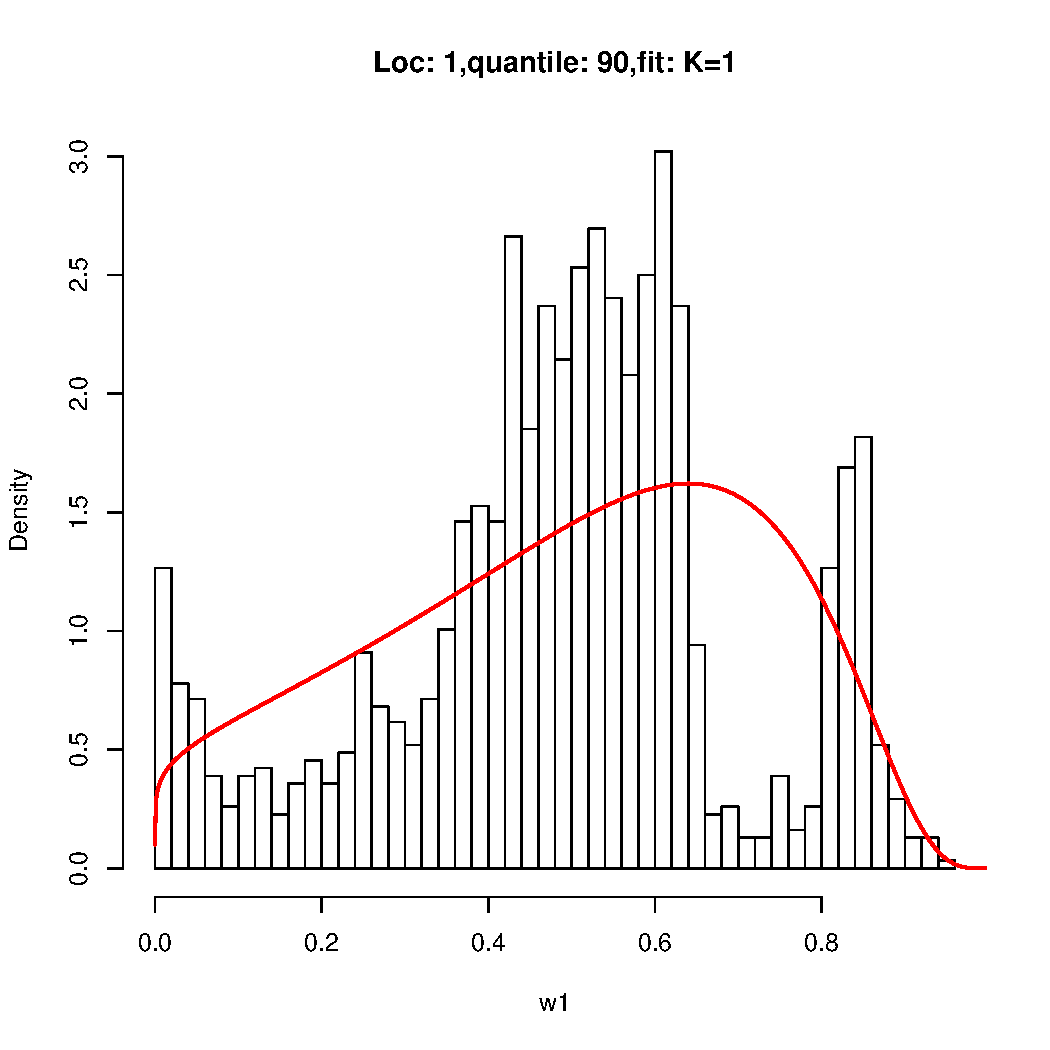
\includegraphics[width=\textwidth/3]{../img/loc1/quantile90/fit_K1.pdf}
&
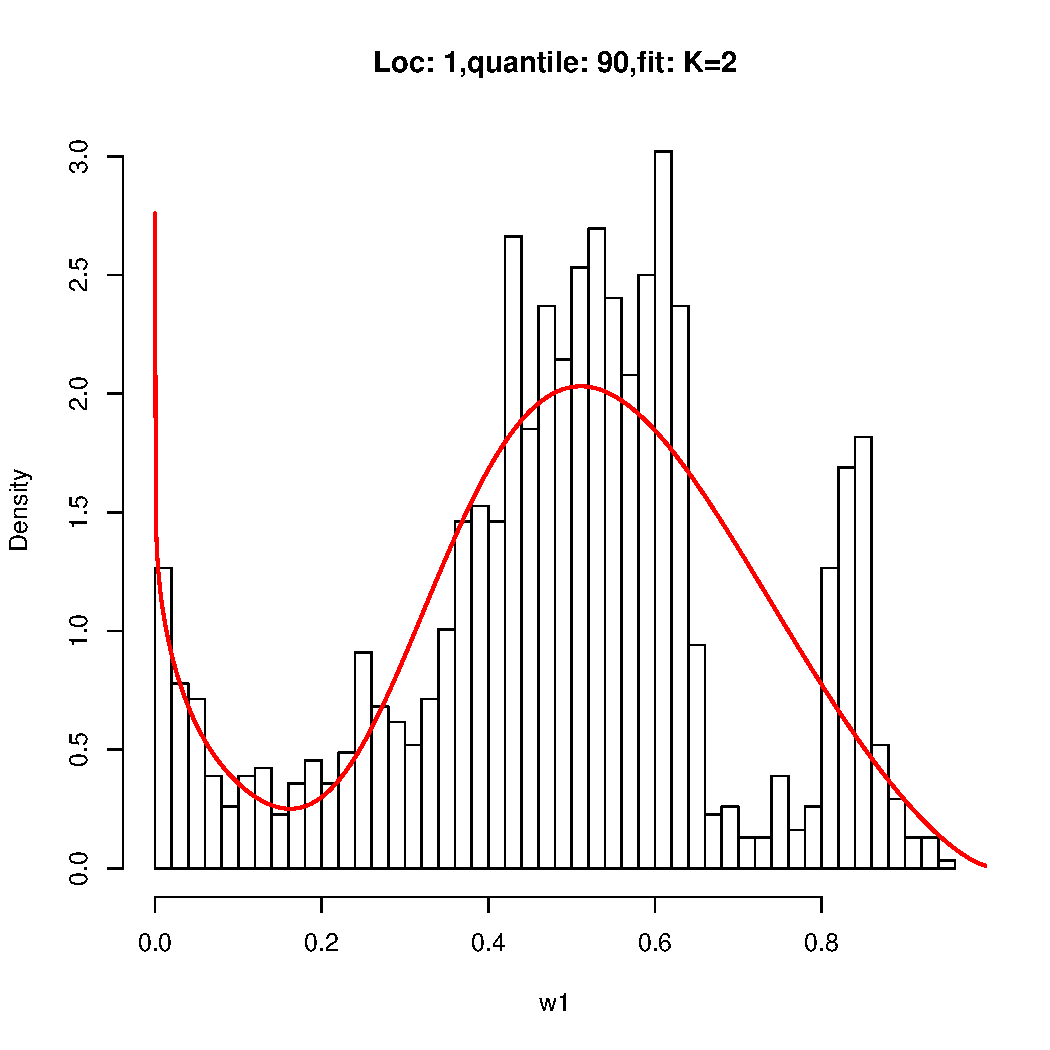
\includegraphics[width=\textwidth/3]{../img/loc1/quantile90/fit_K2.pdf}
&
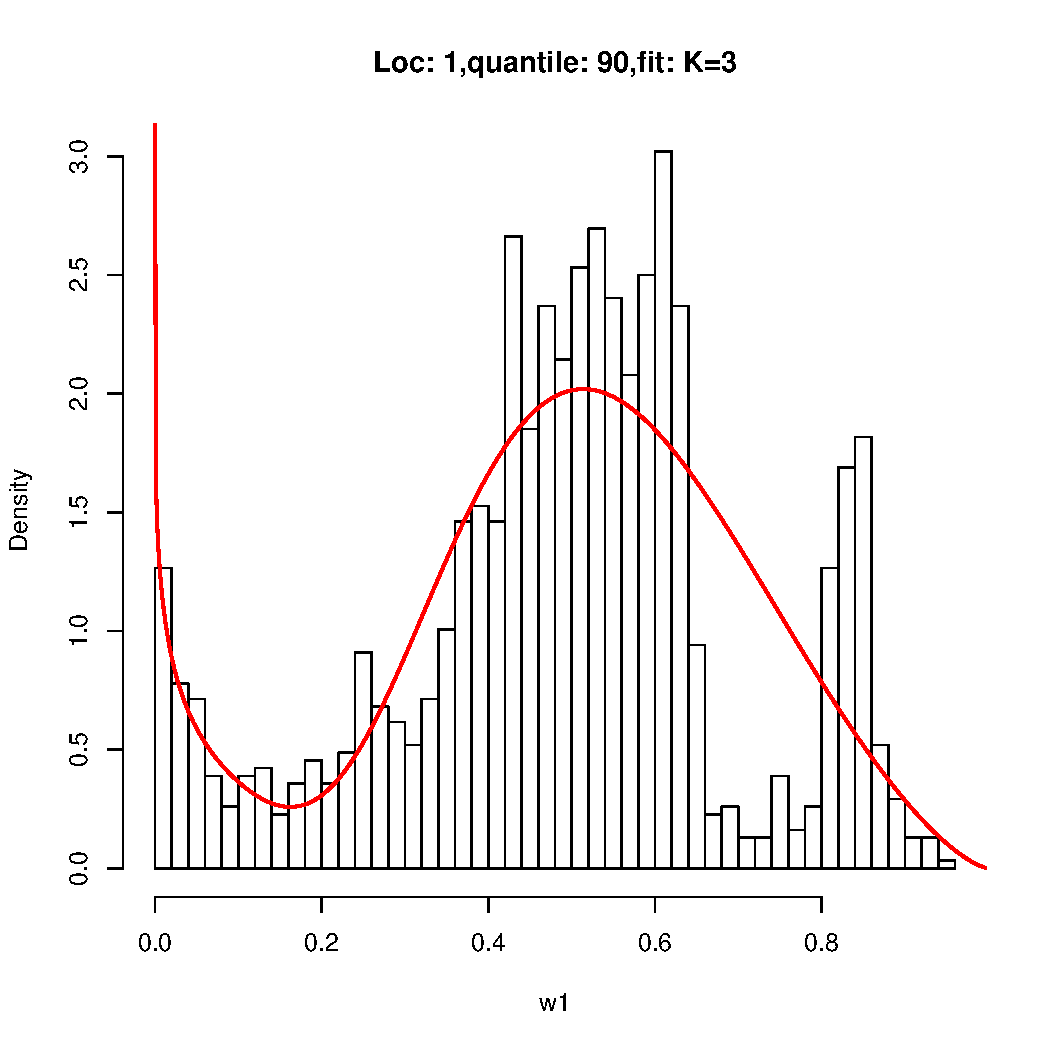
\includegraphics[width=\textwidth/3]{../img/loc1/quantile90/fit_K3.pdf}\\


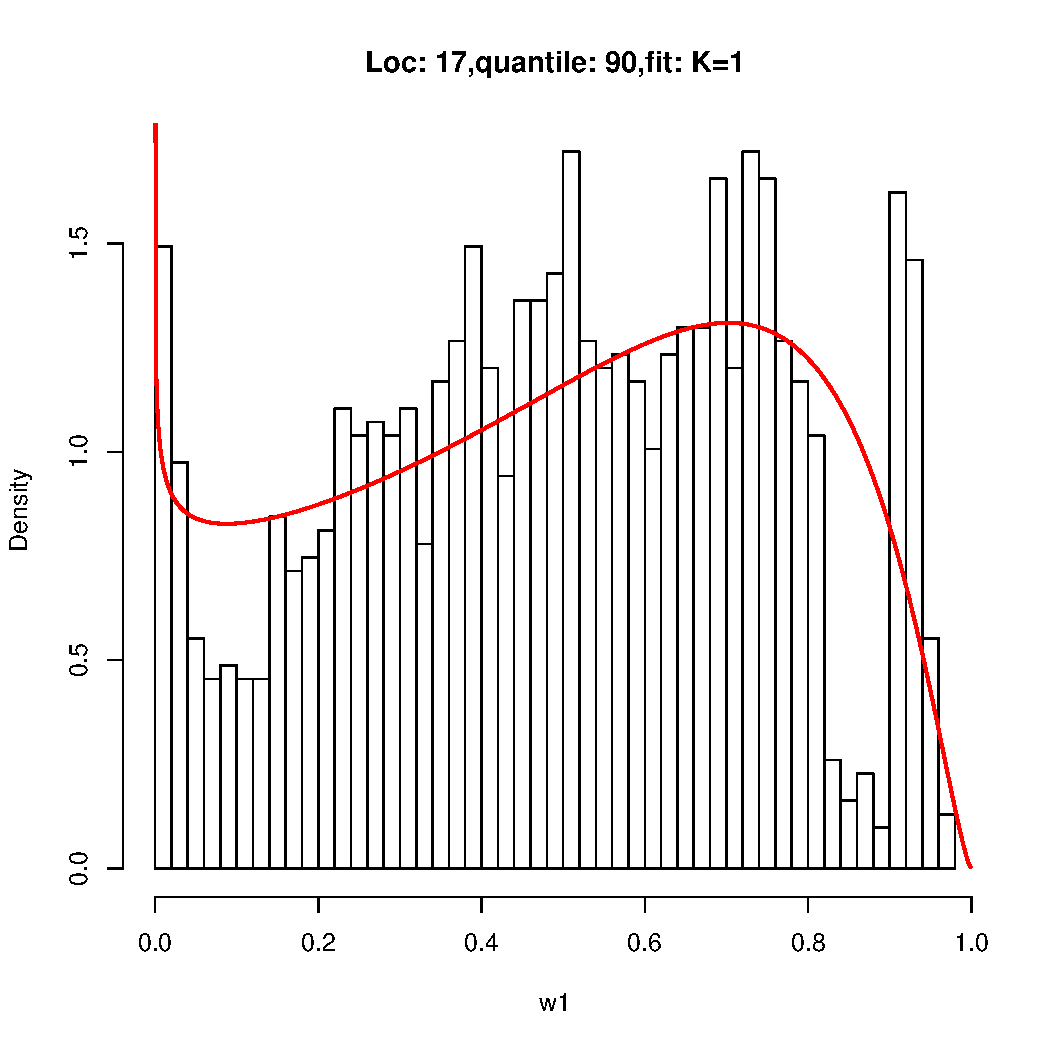
\includegraphics[width=\textwidth/3]{../img/loc17/quantile90/fit_K1.pdf}
&
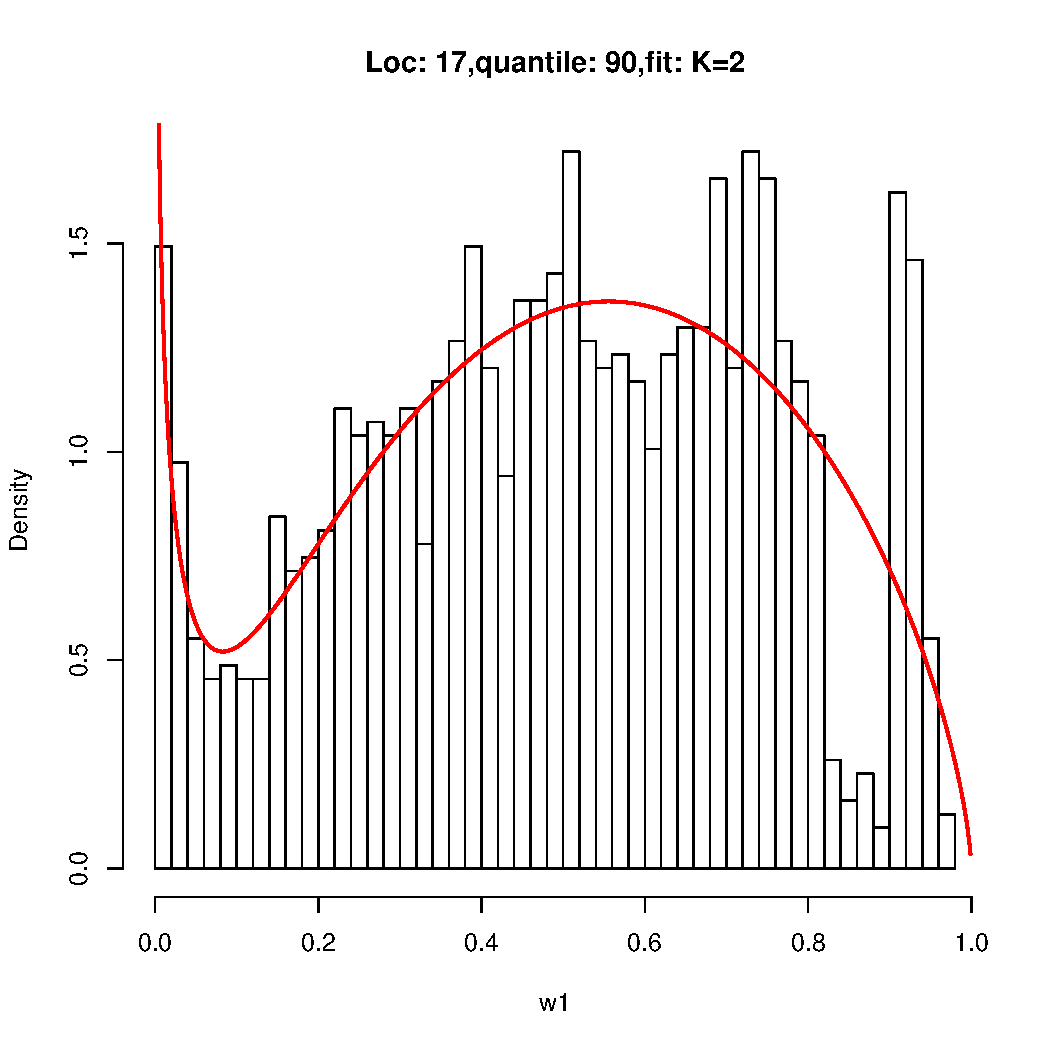
\includegraphics[width=\textwidth/3]{../img/loc17/quantile90/fit_K2.pdf}
&
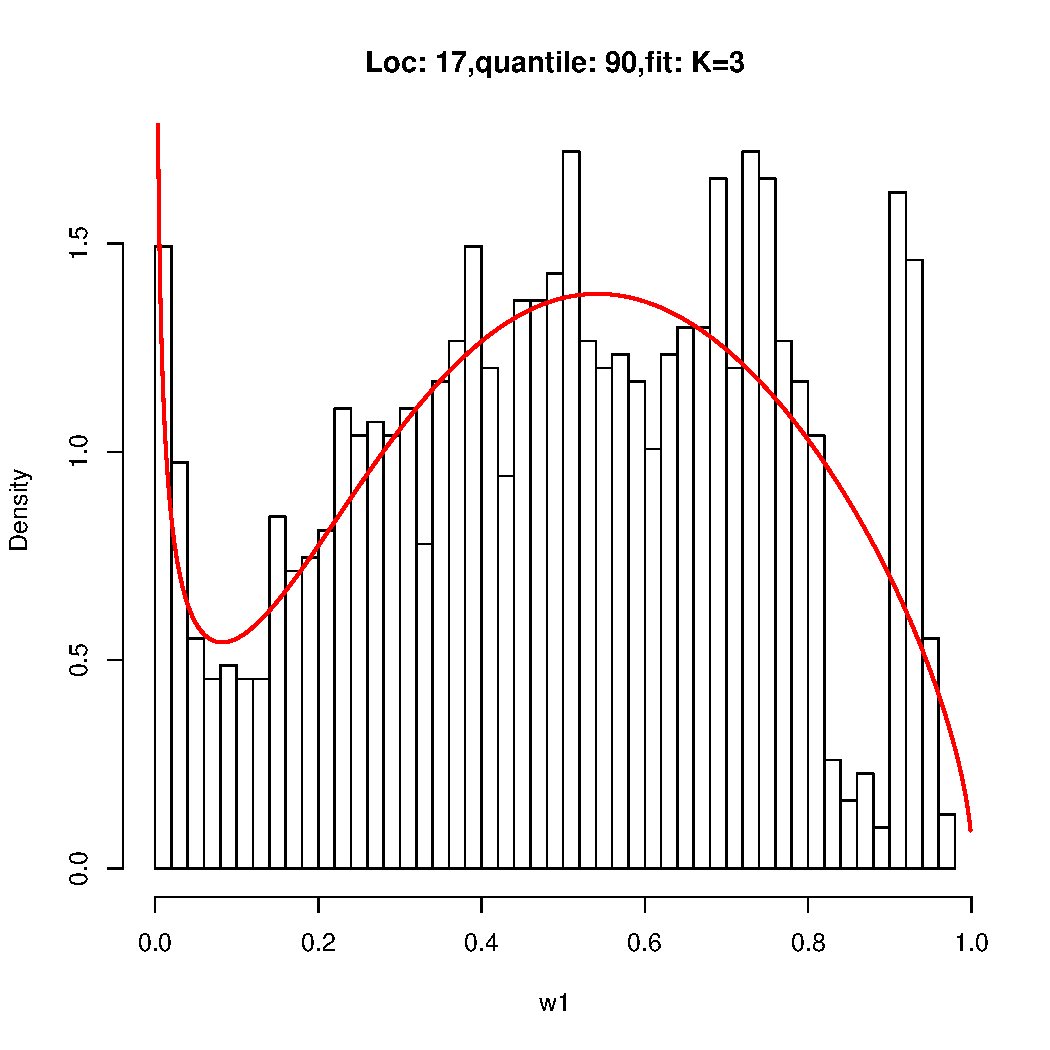
\includegraphics[width=\textwidth/3]{../img/loc17/quantile90/fit_K3.pdf}\\


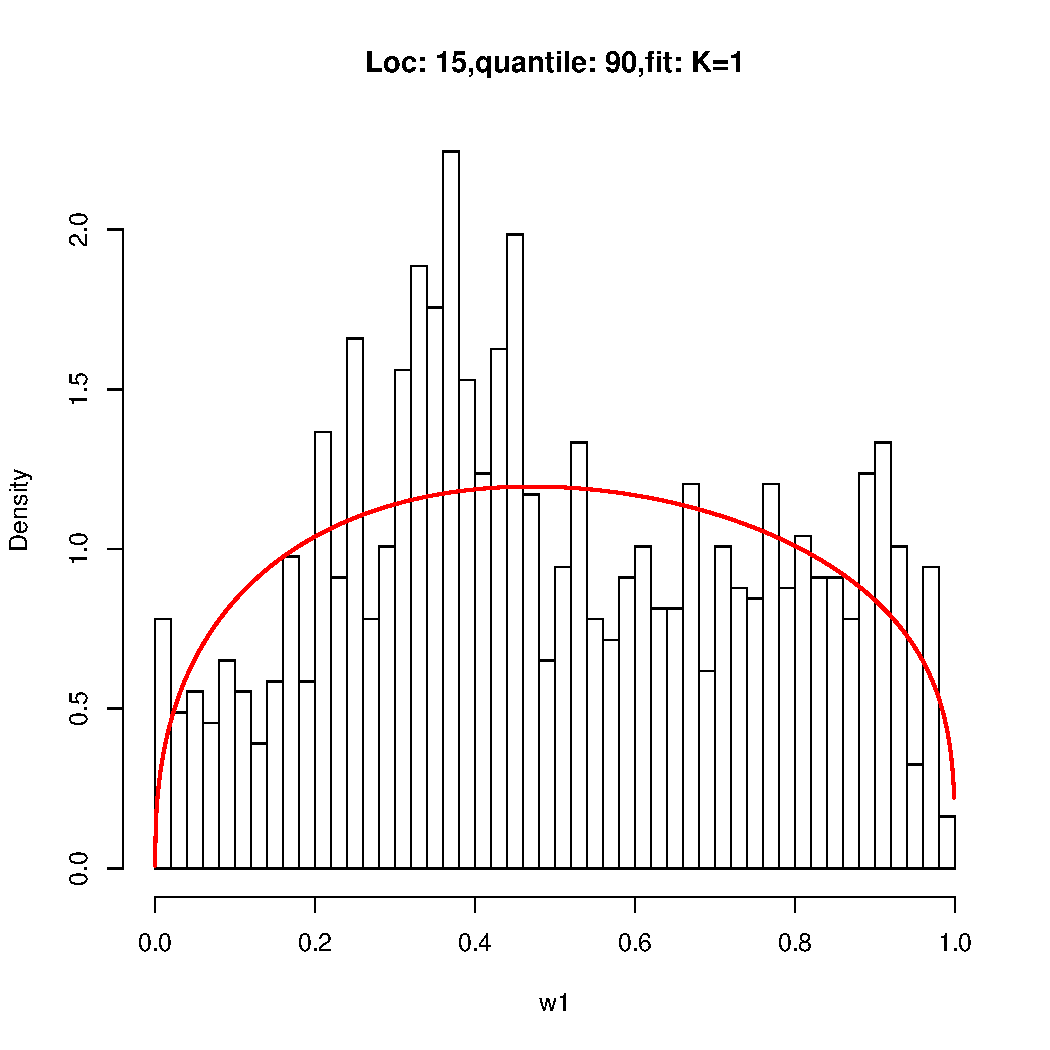
\includegraphics[width=\textwidth/3]{../img/loc15/quantile90/fit_K1.pdf}
&
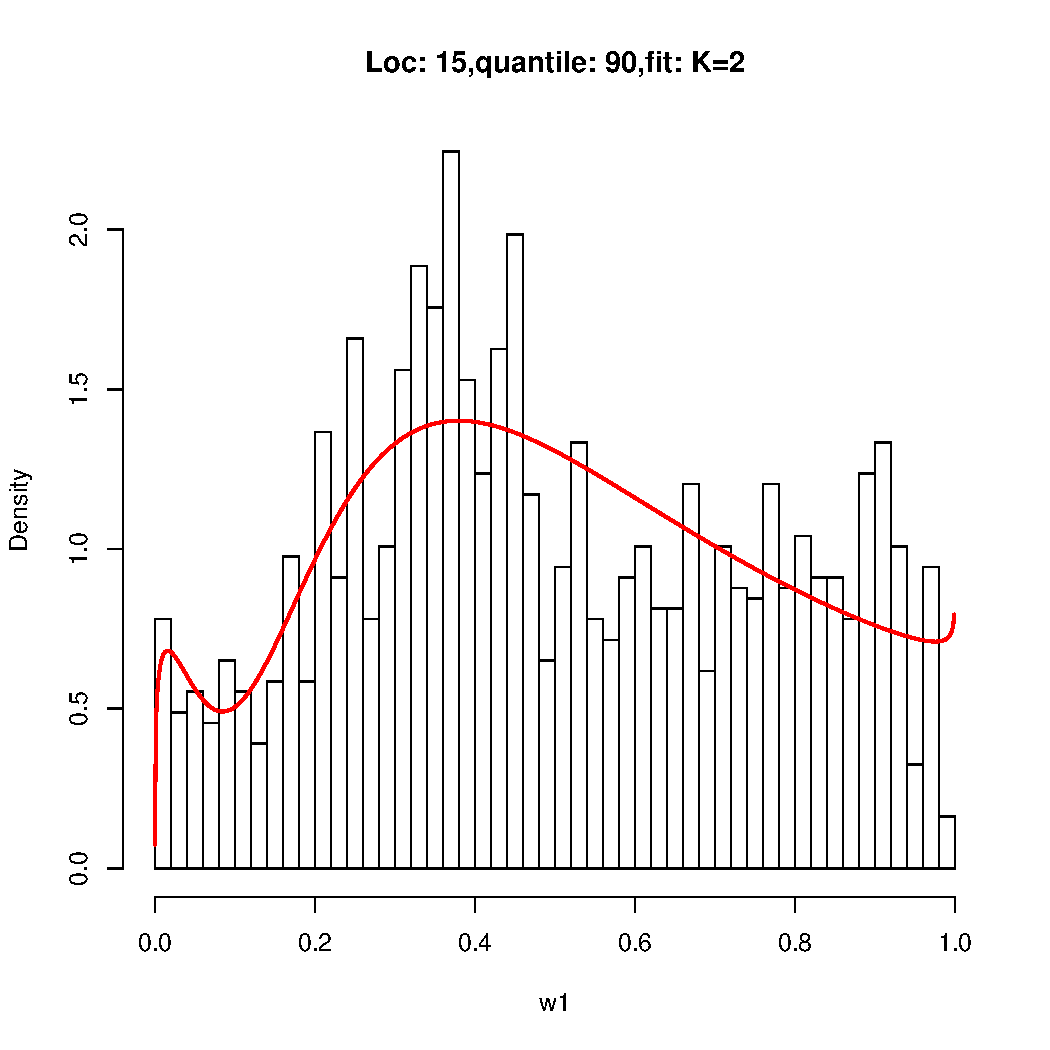
\includegraphics[width=\textwidth/3]{../img/loc15/quantile90/fit_K2.pdf}
&
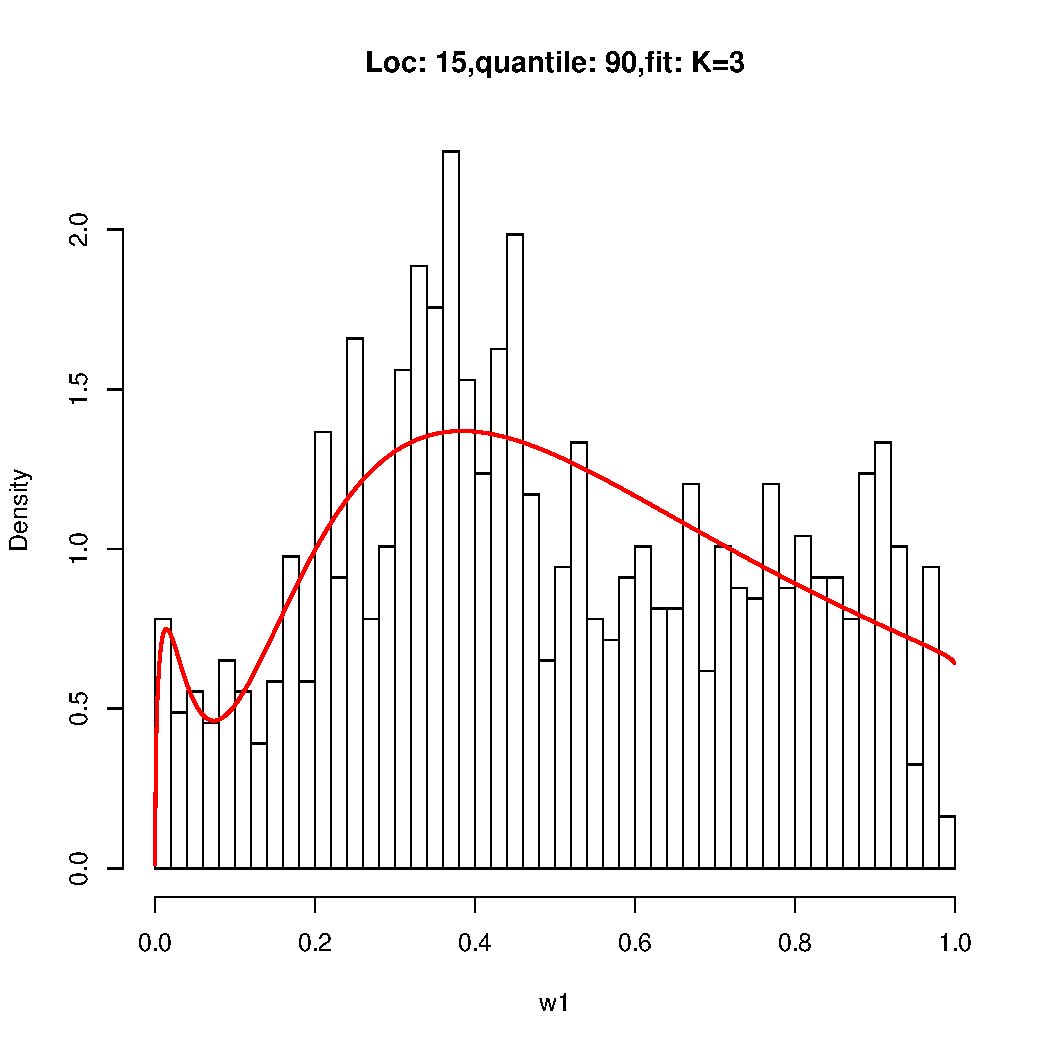
\includegraphics[width=\textwidth/3]{../img/loc15/quantile90/fit_K3.pdf}\\
\end{tabular}
\caption{Fits to locations 1, 17 and 15, using from left to right $K=1,2,3$. The graphs are zoomed in, as nothing interesting is happening outside of this range.}
\label{fig:data_fit}
\end{figure}


We can see graphically the result of fitting tilted mixtures to locations 1,17 and 15 using 1,2, and 3 components in Figure \ref{fig:data_fit}. Visually there seems to be a big improvement between $K=1$ and $K=2$ but then hardly any improvement between 2 and 3 component fits, suggesting that there is no extra gain in using 3 component versus using only 2. Quantitatively, looking at Table \ref{table:estimates}, we see that a forward step-AIC method would also chose the models with $K=2$. So it would seem that using 2 components is the way to go here. However there is an issue: the \texttt{Nelder-Mead} reached the maximum number of iterations, which is set at 1'000, before converging already in the cases $K=2$, which means that the fact that the 3 component cases have higher AIC may just be that we didn't give it enough time, and as it has to fit more 3 extra parameters it is penalized more while not getting to it's peak Likelihood.
We could just up the maximum number of iterations, but instead we are going to keep the maximum number of iterations the same, but switch from the \texttt{Nelder-Mead} optimiser to the \texttt{BFGS} optimizer, which is a little more aggressive in it's exploration of the parameter space. This means that it will take bigger steps towards convergence, but might be more unstable.



\begin{table}
\centering
\begin{tabular}{ |c|c|c||c|c|c||c|c|c||c|c|c| } 
\hline
Loc & K & AIC & $\hat\pi_1$ & $\hat\alpha_1$ & $\hat\beta_1$
& $\hat\pi_2$ & $\hat\alpha_2$ & $\hat\beta_2$
& $\hat\pi_3$ & $\hat\alpha_3$ & $\hat\beta_3$\\
\hline
 \hline
1 & 1 & -458 & 1 & 1.15 & 5.83
& & &
& & & \\

1 & 2 & -711 & 0.94 & 15.42 &  2.4
& 0.06 & 0.91 & 0.95
& & &\\

1 & 3 & -705 & 0.94 & 13.67 & 2.41
& 0.03 & 0.89 &  3.5
& 0.03 & 2.55 & 2.53 \\
\hline
17 & 1 & -147 & 1 & 0.88 & 2.41
& & &
& & &\\

17 & 2 & -194 & 0.94 & 2.17 & 1.68
 &  0.06 & 0.67  & 14.01
 & & &\\
 
17 & 3 & -185 & 0.17  &  0.57  &   0.99
& 0.71  & 3.06 & 1.68
 & 0.12 & 4.12 & 1.55\\
 \hline
15 & 1 & -79 & 1 & 1.4 & 1.29
& & &
& & &\\

15 & 2 & -116 & 0.067 & 1.26 & 0.67
& 0.93 & 8.22 & 0.97
& & &\\

15 & 3 & -110 & 0.91 & 5.17 & 1.01
& 0.07 & 2.13 & 0.95
&  0.02 & 1.48  & 7.63 \\
 \hline
\end{tabular}
\caption{MLE estimates for locations 1,17 and 15, using K=1,2 and 3 components, with \texttt{Nelder-Mead} using maximum 1000 iterations.}
\label{table:estimates}
\end{table}

%K3 loc 1 AIC -1029.6813453965
%K4 loc 1 AIC -1070.60708708505
%K5 loc 1 AIC -1073.64455065985
%K6 loc 1 AIC -1093.31684082104
%K7 loc 1 AIC -1081.75167135068

%K3 loc17 AIC -188.413362805396
%K4 loc17 AIC -186.111154454565
%K5 loc17 AIC -198.220480100418
%K6 loc17 AIC -350.716244649545

%K3 loc15 AIC -111.903125507642
%K4 loc15 AIC -105.90322767153
%K5 loc15 AIC -99.9032260849303
%K6 loc15 AIC -93.9032295849453

In Table \ref{table:AIC} we can see the AIC value for mixtures with more components, using \texttt{BFGS} with a maximum of 1'000 iterations. For location 1, we do indeed see that using more components yields quite a bit better AIC value compared to $K=2$ in Table \ref{table:estimates} and a forward step-AIC method would chose $K=6$. For locations 17 and 15 however, the AIC is smaller for $K=3$, even using \texttt{BFGS} compared to $K=2$ using \texttt{Nelder-Mead} and forward step-AIC methods would still keep $K=2$. We can see that if we skip a few $K$s the AIC start decreasing again, even massively between $K=5$ and $K=6$ for location 17. Looking at the graphs of the fit, this is probably due to overfitting. 
As for location 15, we see that the AIC increases by 6 for every added component, which means that the minimum negative log likelihood is not changing at all, while the penalty for parameter increases (${\rm AIC} = 2(3K-1) - 2\log(L)$)

For the rest of the analysis, we shall use the fits with 6, 2 and 2 components respectively for locations 1, 17 and 15.

\begin{table}
\centering
\begin{tabular}{|c||c|c|c|c|c|}
\hline
loc & K=3 & K=4 & K=5 & K=6 & K=7\\
\hline
1 & -1029 & -1070 & -1073 & -1093 & -1081 \\
17 & -188 & -186 & -198 & -350 & \\
15 & -112 & -106 & -100 & -94 & \\
\hline
\end{tabular}
\caption{AIC for fits using \texttt{BFGS} for various number of components}
\label{table:AIC}
\end{table}

\subsubsection{Goodness of fit}
To check the goodness of fit, we will do several statistical test. The first test we will do, it a Kolmogorov-Smirnov test to see if it is plausible that the data came from the tilted mixtures we selected above. The KS test will test the null hypothesis that this is the case, versus the alternative hypothesis that it does not come from the selected tilted mixture.



For location 17, the model is a tilt of $0.94Beta(2.08,1.71) + 0.06Beta(0.67, 16.33)$. The KS test gives us a p-value of $0.056$. This is low, but depending on what level we chose this could be significant or not.
%D = 0.036703, p-value = 0.05588

For location 15, the model is a tilt of $0.95Beta(7.77,0.98) + 0.05Beta(1.25,1.04)$. The KS test gives a p-value of $0.059$. This is low, but depending on what level we chose this could be significant or not.
%D = 0.042725, p-value = 0.05935


For location 1.
There is a problem with this model, in that it has means $m_1 \approx 0$ and $m_2 \approx 1$ such that it is impossible to sample from this distribution in \texttt{R} using the method in Section \ref{sec:tilting} because the value $m_{\min}/m^Tw \approx 0$ and the acceptance rate is for all intent and purposes, zero. A KS test using the \texttt{ks.test()} command cannot be done.
Switching back to the model were $K=3$, which has the most significance increase in its AIC when adding a component, we get a p-value of $0.059$ for the KS test. This is low, but depending on what level we chose this could be significant or not.
A model with a higher $K$ might be better.
%D = 0.0346, p-value = 0.05947


The problem with the KS test in \texttt{R} is that it uses samples from the null distribution, which means that the p-value will vary for every sample (and sample sizes), making the value not particularly useful. I have set a seed in \texttt{R} for reproducibility. What might be better, is to do the test over and over so many times, than take the mean p-value. It may just be here that I took too many sample of the null distribution ($\approx 100 \times$ as many as in the fitted data)

\chapter{Conclusions}

\begin{thebibliography}{9}

\bibitem{ColesTawn}
S. Coles and J. A. Tawn, \textit{Modelling Extreme Multivariate Events}, Journal of the Royal Statistical Society, 1991, pp. 381-382

\bibitem{Coles}
S. Coles, \textit{An Introduction to Statistical Modelling of Extreme Values}, Springer Series in Statistics, 2001, p. 144


\bibitem{BoldiDavison}
M.-O. Boldi and A. C. Davison, \textit{A mixture model for multivariate extremes}, Journal of the Royal Statistical Society Series B,  2007, pp.217-218

\end{thebibliography}


\chapter*{Code}



%\printindex

\end{document}
